\documentclass[a4paper,11pt,twoside,openright]{article} %wersja do druku
\usepackage[T1]{fontenc}
\usepackage[english,polish]{babel}
\usepackage[utf8]{inputenc}
\usepackage{lmodern}
\selectlanguage{polish}
\usepackage[left=2.0cm, right=2.0cm, top=2.5cm, bottom=2.5cm]{geometry}
\usepackage{latexsym}
\usepackage{graphicx}
\usepackage{amsmath}
\usepackage{enumerate}
\usepackage{bm}
\usepackage{tikz}
\usepackage{float}
\usetikzlibrary{matrix,shapes,arrows,positioning,chains,intersections}
\usepackage{multirow}
\usepackage{bm}
\usepackage{smartdiagram}
\usepackage{textcomp}
%\usetikzlibrary{shapes,arrows}
\usepackage{tikz}
\usetikzlibrary{graphs}
\usepackage{forest}
\usetikzlibrary{automata,positioning} %to chyba nie dziala, mialo zawijac tekst w drzewku
\usepackage{chngcntr} %to i nizej sa od numerowania rysunkow zgodnie z rozdzialem
\counterwithin{figure}{section} 
\usepackage{textcomp} %greckie literki w tekscie
\usepackage{graphicx} %foty
\usepackage{wrapfig} %zawijanie tekstu 
\usepackage{enumerate} %prosta lista
\usepackage[nottoc,numbib]{tocbibind} %biblio w ToC
%\usepackage{tabu} %grubosc lini w tabeli
\usepackage{chngcntr} %numerowanie tabeli zgodnie z numerem rozdzialu (to nizej tez)
\counterwithin{table}{section} %numerowanie tabel zgodnie z numerem rozdzialu
\usepackage[toc,page]{appendix} %anex
\usepackage{adjustbox} %ograniczenie tabelek do wielkosci strony
\usepackage{pdfpages}

\newsavebox{\temp}
\newlength{\tempwidth}
\newlength{\tempheight}

\newcommand{\addpdf}[1]{%
    \sbox{\temp}{\includegraphics{#1}}%
    \setlength{\tempwidth}{\widthof{\usebox{\temp}}}%
    \setlength{\tempheight}{\heightof{\usebox{\temp}}}%

    \ifthenelse{\tempwidth > \tempheight}
        {\includepdf[fitpaper, templatesize={210mm}{297mm}, scale=0.92, landscape]{#1}}
        {\includepdf[fitpaper, templatesize={210mm}{297mm}, scale=0.92]{#1}}%
}

\newcommand{\myTitle}{KAP_laboratorium_3}
\newcommand{\myName}{Paweł Gilewicz}
\newcommand{\myThesisType}{Sprawozdanie}

% apply config to document settings
\title{\myTitle}
\author{\myName}
\usepackage[unicode, hidelinks]{hyperref}
\hypersetup{
	pdftitle={\myTitle},
	pdfauthor = {\myName},
	pdfsubject={\myThesisType},
	pdfproducer={LaTeX},
	pdfcreator={pdflatex},
	colorlinks=false
}

% MATRIX settings
\usepackage{amsmath}
\makeatletter
\renewcommand*\env@matrix[1][\arraystretch]{%
  \edef\arraystretch{#1}%
  \hskip -\arraycolsep
  \let\@ifnextchar\new@ifnextchar
  \array{*\c@MaxMatrixCols c}}
\makeatother
\usepackage{mathtools}
\usepackage{amsmath}

% DOCUMENT settings
% dot after section/subsection/subsubsection number
\usepackage{secdot}
\sectiondot{subsection}
\sectiondot{subsubsection}

\usepackage{tocloft} %kropki w spisie tresci
\usepackage[labelsep=period]{caption}
\usepackage{graphicx}
\usepackage[font=small, % equivalent to 10 pt font
			labelfont=bf, 
			justification=justified, 
			singlelinecheck=false]{caption} 
\usepackage[justification=centering]{subcaption} % two images side by side captions
\usepackage{booktabs} % pretty LaTeX tables
\usepackage{siunitx} % units SI e.g. \SI{10}{\kilogram\per\meter\square}
\usepackage{mathtools} % amsmath, symbols such as brackets, arrows, equation numbering only for referrenced eqs.
%\usepackage[parfill]{parskip} % spacing between paragraphs instead of indent
%\parfillskip 0pt plus 0.75\textwidth % get rid of widows at the end of paragraphs
\frenchspacing % for "Polish" spaces after the sentence
\usepackage{polski} % Polish rules of hyphenation
\usepackage{dashrule} % for dotted lines in declarations page
\usepackage{emptypage} % removes headers on empty pages
\usepackage{colortbl}

% FONT settings
\usepackage[T1]{fontenc}
\usepackage{helvet} % you can change to 'helvet' for Helvetica clone, 'uarial' for Arial clone, 'lmodern' for Latin Modern
\renewcommand{\familydefault}{\sfdefault} % change font to sans serif
\usepackage{amsfonts} % mathematical fonts
\usepackage{inconsolata} % monospaced font in urls and \texttt
%\usepackage{url}
%\urlstyle{same}

% DEBUG
\usepackage{lipsum}
\usepackage{etoolbox} % removes page number in table of contents
\patchcmd{\chapter}{plain}{empty}{}{}
\usepackage{slantsc}

\usepackage{fancyhdr}%numerki do dwustronnego
\fancyhf{}
\renewcommand{\headrulewidth}{0pt}
\fancyfoot[LE,RO]{\thepage}
\pagestyle{fancy}



\usepackage{animate}
\usepackage{graphicx}
\usepackage{media9}
\usepackage{xkeyval}
\usepackage[T1]{fontenc}
\usepackage[polish]{babel}
\usepackage[utf8]{inputenc}

\usepackage{listings}
\usepackage{xcolor}

\definecolor{codegreen}{rgb}{0,0.6,0}
\definecolor{codegray}{rgb}{0.5,0.5,0.5}
\definecolor{codepurple}{rgb}{0.58,0,0.82}
\definecolor{backcolour}{rgb}{0.95,0.95,0.92}

\lstdefinestyle{mystyle}{
%    backgroundcolor=\color{backcolour},   
    commentstyle=\color{codegreen},
    keywordstyle=\color{magenta},
    numberstyle=\tiny\color{codegray},
    stringstyle=\color{codepurple},
    basicstyle=\ttfamily\footnotesize,
    breakatwhitespace=false,         
    breaklines=true,                 
    captionpos=b,                    
    keepspaces=true,                 
    numbers=left,                    
    numbersep=5pt,                  
    showspaces=false,                
    showstringspaces=false,
    showtabs=false,                  
    tabsize=2
}

\lstset{style=mystyle}



\title{}
\author{}
\date{}

\usepackage{fancyhdr} 
\pagestyle{fancy}
\fancyhf{}
\renewcommand{\headrulewidth}{0.4pt}% Default \headrulewidth is 0.4pt
\rfoot{\thepage}
\rhead{Przejściowa Praca Magisterska}
\lhead{Zakład Aerodynamiki}


\begin{document}
\renewcommand{\figurename}{Rys.} %podpis do rysunku Rys. zamiast Rysunek
\renewcommand{\tablename}{Tab.}
%\maketitle

\section{Przegląd zastosowanych bibliotek}
\subsection{OpenCV}
\noindent \textbf{OpenCV} (Open Source Computer Vision Library) to biblioteka oprogramowania do przetwarzania grafiki komputerowej i uczenia maszynowego. OpenCV został zbudowany w celu zapewnienia wspólnej infrastruktury dla aplikacji z zakresu wizji komputerowej oraz przyspieszenia wykorzystania percepcji maszynowej w produktach komercyjnych. Biblioteka jest wieloplatformowa i licencjonowana jako bezpłatne oprogramowanie typu open source w ramach licencji Apache 2. W pracy OpenCV zastosowano do procesu przetwarzania danych pomiarowych (thresholding, detekcja konturów, stabilizacja obrazu). Zastosowane funkcje zostaną opisane w następnych rozdziałach.

\subsection{SciPy}
\noindent SciPy to bezpłatna biblioteka Pythona o otwartym kodzie źródłowym, używana do obliczeń naukowych i technicznych. Zawiera moduły do optymalizacji, algebry liniowej, integracji, interpolacji, funkcji specjalnych, FFT, przetwarzania sygnału i obrazu, solverów ODE i innych zadań powszechnych w nauce i inżynierii. Biblioteka SciPy jest obecnie dystrybuowana na licencji BSD, a jej rozwój jest sponsorowany i wspierany przez otwartą społeczność programistów
W pracy wykorzystano algorytmy dyskretnej transformaty Fouriera oraz procedury całkowania numerycznego. 

\subsection{NumPy}
\noindent  NumPy to biblioteka dla języka programowania Python, dodająca obsługę dużych, wielowymiarowych tablic i macierzy, wraz z dużym zbiorem funkcji matematycznych wysokiego poziomu do operowania na tych tablicach. NumPy celuje w referencyjną implementację CPython Pythona, która jest nieoptymalizującym interpreterem kodu bajtowego. Używanie NumPy w Pythonie zapewnia funkcjonalność porównywalną z MATLAB -em, ponieważ oba są interpretowane i oba pozwalają użytkownikowi pisać wydajne programy, o ile większość operacji działa na tablicach lub macierzach zamiast na skalarach. Powiązania Pythona z używaną biblioteką komputerową OpenCV wykorzystują tablice NumPy do przechowywania danych i operowania na nich. Ponieważ obrazy z wieloma kanałami są po prostu reprezentowane jako trójwymiarowe tablice, indeksowanie, cięcie lub maskowanie za pomocą innych tablic to bardzo wydajne sposoby uzyskiwania dostępu do określonych pikseli obrazu. Algorytm przetwarzania danych został więc w większości napisany z wykorzystaniem struktury danych biblioteki NumPy.

\subsection{Matplotlib}
\noindent Matplotlib to oparta na języku Python biblioteka do wizualizacji z pełną obsługą grafiki 2D i ograniczoną obsługą grafiki 3D, szeroko stosowana w naukowej społeczności komputerowej Pythona. Biblioteka jest ukierunkowana na szeroki zakres przypadków użycia. Może osadzać grafikę w wybranym zestawie narzędzi interfejsu użytkownika i obecnie obsługuje grafikę interaktywną we wszystkich głównych systemach operacyjnych przy użyciu zestawów narzędzi GTK+, Qt, Tk, FLTK, wxWidgets i Cocoa. Można go wywoływać z interaktywnej powłoki Pythona w celu tworzenia grafiki za pomocą prostych, proceduralnych poleceń, podobnie jak Mathematica, IDL lub MATLAB. Bibliotekę zastosowano do wizualizacji danych.

\newpage

\section{Proces przetwarzania obrazu}
\subsection{Thresholding}
\noindent Proces przetwarzania obrazu rozpoczęto od wczytania danych w sposób umożliwiający wykonywanie operacji na konturach badanych obiektów. Zastosowano technikę znaną powszechnie jako thresholding (progowanie). Ta podstawowa technika segmentacji umożliwia separację pierwszego planu (tj. interesujących nas obiektów) od tła obrazu. Thresholding to ogólnie rzecz biorąc binaryzacja obrazu, która polega na konwersji obrazu w skali szarości na obraz binarny, w którym piksele mają wartość 0 lub 255. Prostym przykładem thresholdingu byłoby wybranie wartości progowej T, a następnie ustawienie intensywności wszystkich pikseli mniejszych niż T na 0, a wszystkich pikseli większych niż T na 255. W ten sposób tworzy się binarną reprezentację obrazu. Thresholding występuje w trzech formach:
\begin{enumerate}
\item Progowanie binarne/proste (\textit{binary thresholding}), w którym ręcznie ustala się parametry do segmentacji obrazu. Sposób ten działa wyjątkowo dobrze w kontrolowanych warunkach oświetleniowych, w których można zapewnić wysoki kontrast pomiędzy pierwszym planem a tłem obrazu. Warunki takie zapewniono w laboratorium podczas przeprowadzania pomiarów.
\item Progowanie Otsu (\textit{Otsu's thresholding}), zwracające w najprostszej formie pojedynczy próg intensywności, który dzieli piksele na dwie klasy, pierwszy plan i tło. Próg ten jest określany przez minimalizację wariancji intensywności wewnątrz klasy lub równoważnie przez maksymalizację wariancji między klasami.
\item Progowanie adaptacyjne (\textit{adaptive thresholding}). W tym przypadku algorytm określa próg dla piksela na podstawie małego obszaru wokół niego. Otrzymujemy więc różne progi dla różnych obszarów tego samego obrazu, co daje lepsze wyniki dla obrazów o różnym oświetleniu.
\end{enumerate}
\noindent Na rysunku (\ref{fig:raw_data}) przedstawiono reprezentację surowych danych pomiarowych. Pomiędzy obiektem (kroplą) a tłem zapewniony jest wysoki kontrast poprzez kontrolowanie warunków oświetleniowych i ustawień kamery. 
\captionsetup{skip=0pt}
\begin{figure}[!h]
\captionsetup{justification=centering}
\begin{center}
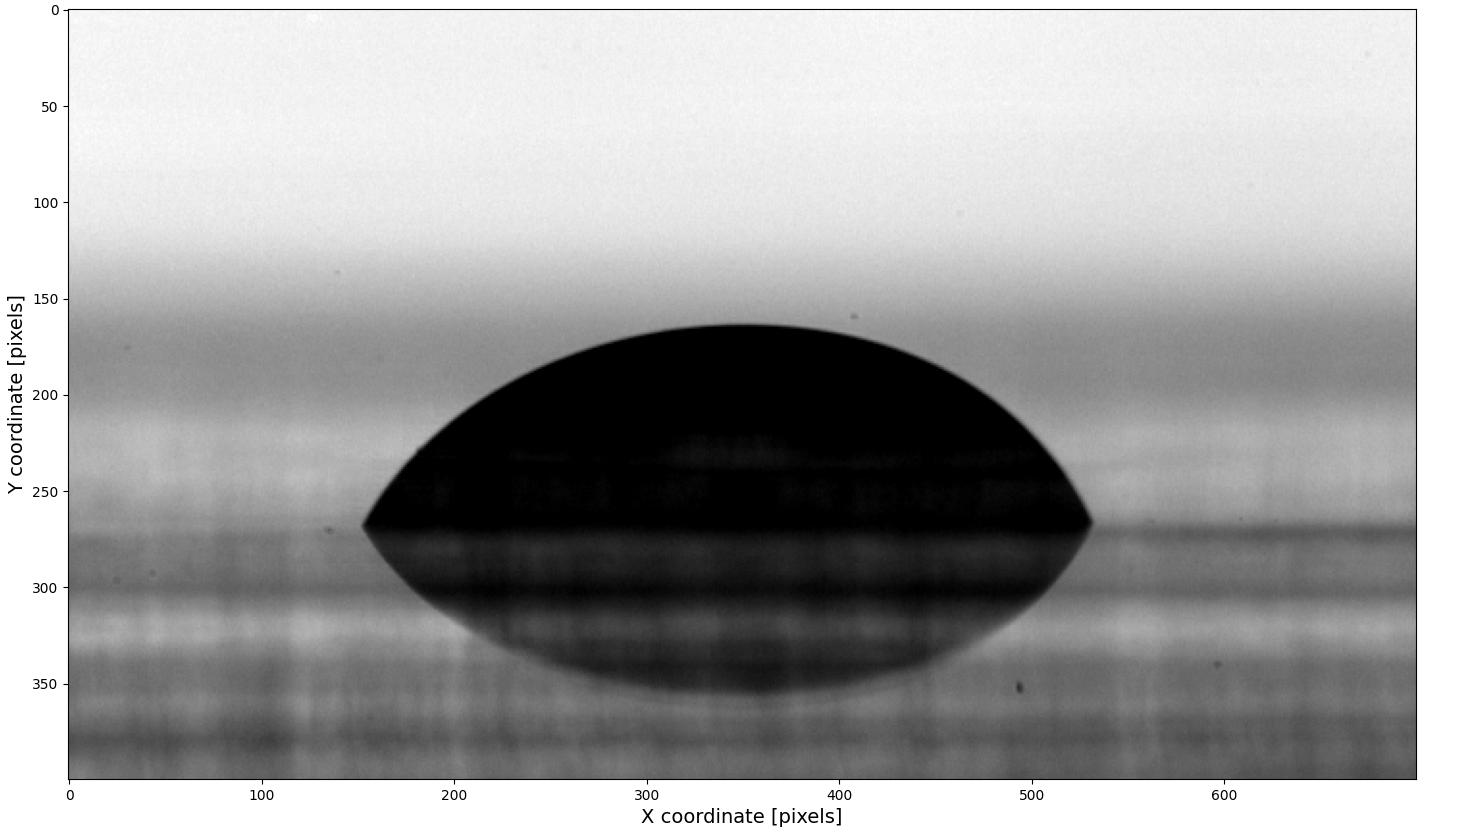
\includegraphics[width=0.9\textwidth]{../workspace/RawData.png} 
\end{center}
\caption{Reprezentacja surowych danych pomiarowych.\\ Wysoki kontrast pomiędzy badanym obiektem a tłem}
\label{fig:raw_data}
\end{figure} 
\newpage

\noindent Przedstawiony na rys. \ref{fig:raw_data} obraz poddano operacji thresholdowania wykorzystując różne algorytmy dostępne w bibliotece \textbf{OpenCV}. Proces ten miał na celu wybór algorytmu, który w danych warunkach najlepiej odwzoruje kształt obiektu. Głównym kryterium oceny zastosowanych algorytmów było to, czy przekonwertowane zdjęcia pokryte są szumem. Poniższy rysunek prezentuje zestawienie efektów.

\captionsetup{skip=0pt}
\begin{figure}[!h]
\captionsetup{justification=centering}
\begin{center}
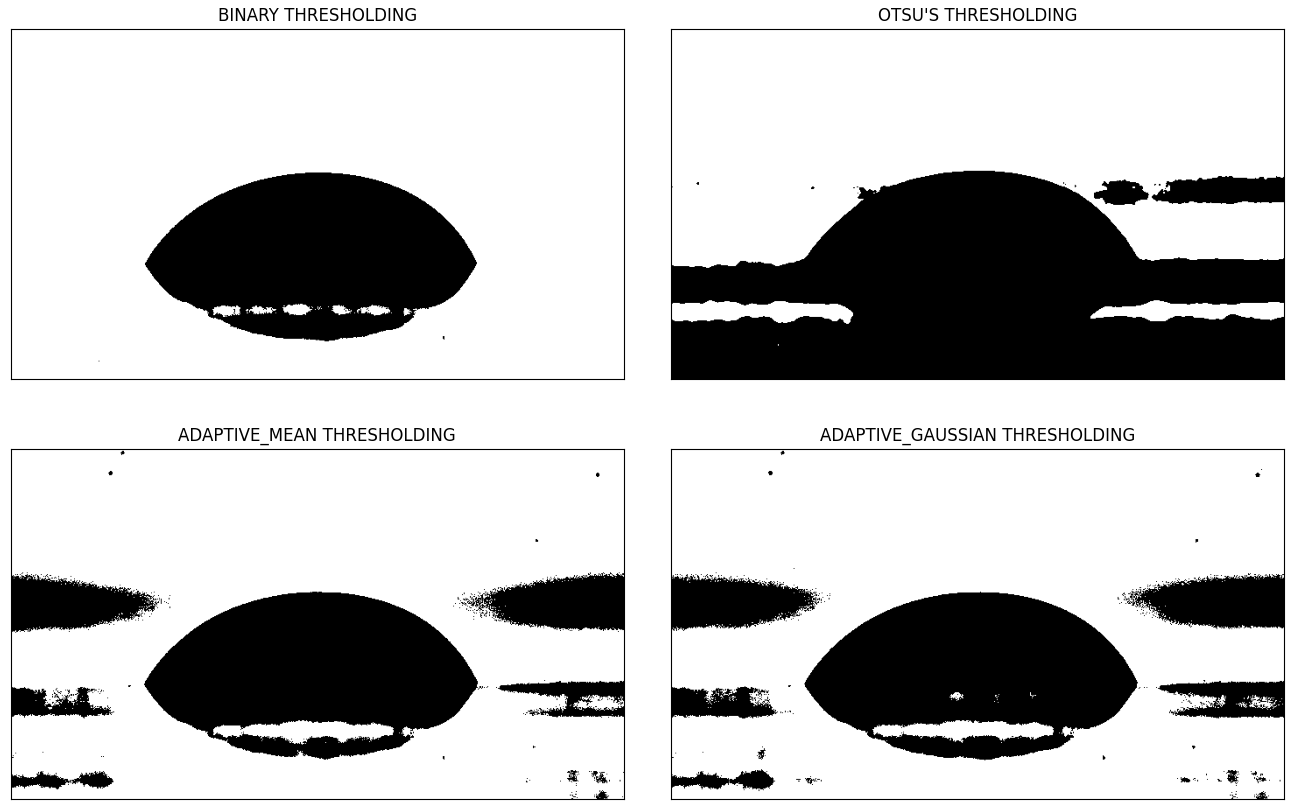
\includegraphics[width=1\textwidth]{../workspace/threshold_comp.png} 
\end{center}
\caption{Zestawienie obrazów otrzymanych w wyniku operacji thresholdowania przy użyciu algorytmów dostępnych w bibliotece \textbf{OpenCV}.}
\label{fig:threshold}
\end{figure} 

\noindent Biorąc pod uwagę fakt, że konwersja dotyczy bardzo dużej ilości zdjęć (sumarycznie liczba ta jest rzędu tysięcy), zastosowany algorytm musi charakteryzować się stabilnością. Rejestrowanie zdjęć z dużą częstością powoduje, że na obrazach widoczne są różnice oświetlenia wynikające z częstotliwości pracy lampy. W związku z tym implementowany algorytm musi być odporny na to zjawisko. Co więcej model numeryczny powinien charakteryzować się łatwą adaptacją do jakości wczytywanych obrazów, tzn. w zależności od ich naświetlenia powinien zwracać zawsze prawidłowy kształt obiektu.
Uwzględniając wszystkie wytyczne, po przeprowadzeniu serii testów, zaimplementowano thresholding binarny, w którym wartość progowa wprowadzana jest przez użytkownika. Zapewnione warunki pomiaru, przy użyciu tego algorytmu pozwalają na konwersję zdjęcia do postaci niezaszumionej, w której kształt obiektu jest dokładnie odwzorowany (rys. \ref{fig:threshold}).

\vspace{10mm}
\subsection{Detekcja konturu kropli} 
\label{chapter:contour_detection}
\noindent Przeprowadzenie operacji binaryzacji obrazu umożliwia dalszą obróbkę zdjęć. W tym podrozdziale opisana zostanie technika detekcji konturu kropli. Kontury można określić jako krzywą łączącą wszystkie ciągłe punkty (wzdłuż granicy), mające ten sam kolor lub intensywność. Zgodnie z taką definicją w bibliotece OpenCV zaimplementowana jest funkcja \textbf{findContours()}, przyjmująca trzy argumenty. Pierwszy z nich to zbinaryzowany obraz źródłowy, drugi to tryb detekcji konturów, a trzeci to metoda aproksymacji. Każdy znaleziony kontur jest zwracany przez funkcję w postaci wektorów współrzędnych (x, y) określających granicę analizowanego obiektu. Tryb detekcji konturów to w praktyce parametr określający postać konturów, którą zwrócić ma funkcja. W szczególności przydatne jest to przy detekcji wielu konturów na raz, jednak w realizowanym przypadku mamy do czynienia tylko z jednym konturem. Co więcej, detekcja więcej niż jednego konturu byłaby niepożądana (traktowalibyśmy to jako szum). W związku z tym jako drugi argument funkcji ustawiono flagę cv2.RETR\_EXTERNAL, co w konsekwencji powoduje zwracanie jednego konturu. Rozważaniom poddano natomiast metodę aproksymacji oraz czułość pomiarów na jej wpływ. Na rysunku \ref{fig:approx_method} przedstawiano kontury otrzymane poprzez aproksymację odpowiednio: metodą cv2.CHAIN\_APPROX\_NONE oraz \\cv2.CHAIN\_APPROX\_SIMPLE. Obie metody zwróciły identyczny wynik.

\captionsetup{skip=0pt}
\begin{figure}[!h]
\captionsetup{justification=centering}
\begin{center}
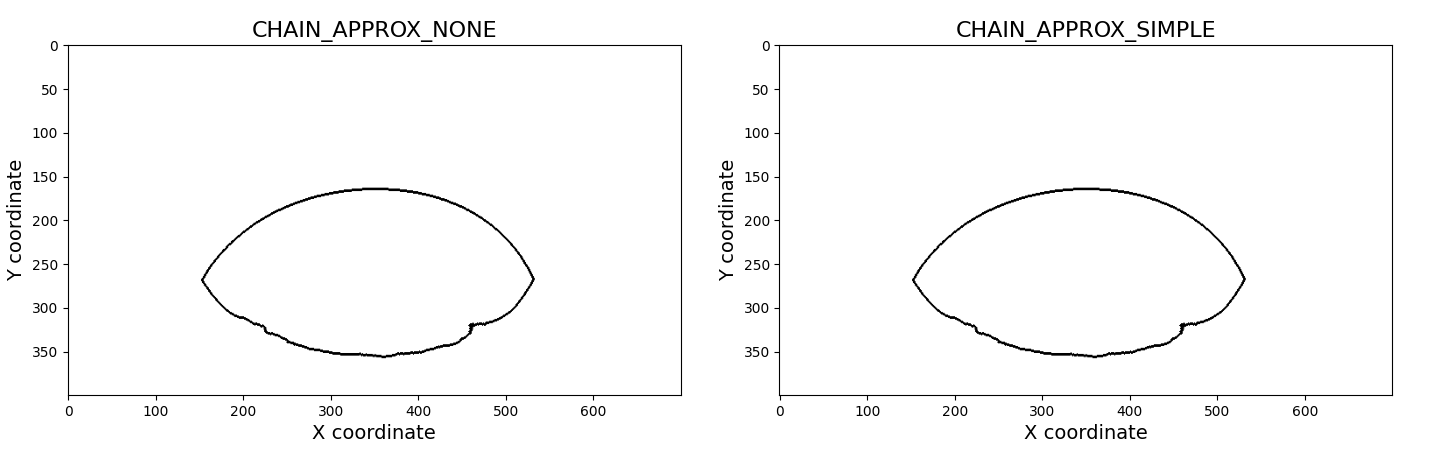
\includegraphics[width=1\textwidth]{../workspace/approximation_chain.png} 
\end{center}
\caption{Zestawienie konturów otrzymanych w wyniku zastosowania metody\\cv2.CHAIN\_APPROX\_NONE (wykres lewy) oraz cv2.CHAIN\_APPROX\_SIMPLE (wykres prawy).}
\label{fig:approx_method}
\end{figure} 

\noindent Przedstawione na powyższym rysunku krzywe to kontury zarówno kropli, jak i rzucanego przez nią cienia. Mając na uwadze fakt, że analizowany jest jedynie kształt kropli, w kolejnych operacjach odcięto obszar reprezentujący cień. Odcięty obszar ogranicza prosta reprezentująca krawędź płytki.

\vspace{10mm}
\subsection{Stabilizacja obrazu}
\noindent W celu lepszej wizualizacji danych pomiarowych oraz na potrzeby dalszego przetwarzania obrazu program wzbogacono o algorytm stabilizacji obrazu, który działa w oparciu o obiekt referencyjny na stałe związany z układem odniesienia płytki. Obiekt ten stanowi drucik uformowany w taki sposób, aby kropla nie znajdowała się w jego śladzie aerodynamicznym (rys. \ref{fig:reference_object}). Rozwiązanie takie wynika z potencjalnego problemu śledzenia obiektu na podstawie krzywej ruchu. Problem ten wynika z konieczności synchronizacji ruchu rejestrowanego przez kamerę z rzeczywistym ruchem płytki. Na rysunku \ref{fig:meas_problem} przedstawiono ideę problemu. Jego źródłem są dwie własności układu pomiarowego:
\begin{enumerate}
	\item Oś optyczna kamery nie przechodzi przez początek układu współrzędnych siłownika. Innymi słowy w pozycji zerowej oś kamery nie pokrywa się z pozycją badanego obiektu. Wprowadza to pewne przesunięcie, które na rys. \ref{fig:meas_problem} zostało oznaczone jako $\Delta$y. Aby pozbyć się tego efektu, każdy pomiar musiałby zostać poprzedzony dokładną kalibracją położenia kamery.
	\item Początek ruchu platformy nie jest zsynchronizowany z rozpoczęciem nagrywania pomiaru. Efekt ten przejawia się jako przesuniecie fazowe, które na rys. \ref{fig:meas_problem} oznaczono jako $\Delta \varphi$. Jest to efekt, który ma zdecydowanie większy wpływ, a jednocześnie jest trudniejszy do wyeliminowania. Potencjalnym sposobem byłaby modyfikacja stanowiska pomiarowego w taki sposób, aby pomiar rozpoczynany był w tym samym  momencie, co ruch platformy.
\end{enumerate}
\newpage

\captionsetup{skip=0pt}
\begin{figure}[!h]
\captionsetup{justification=centering}
\begin{center}
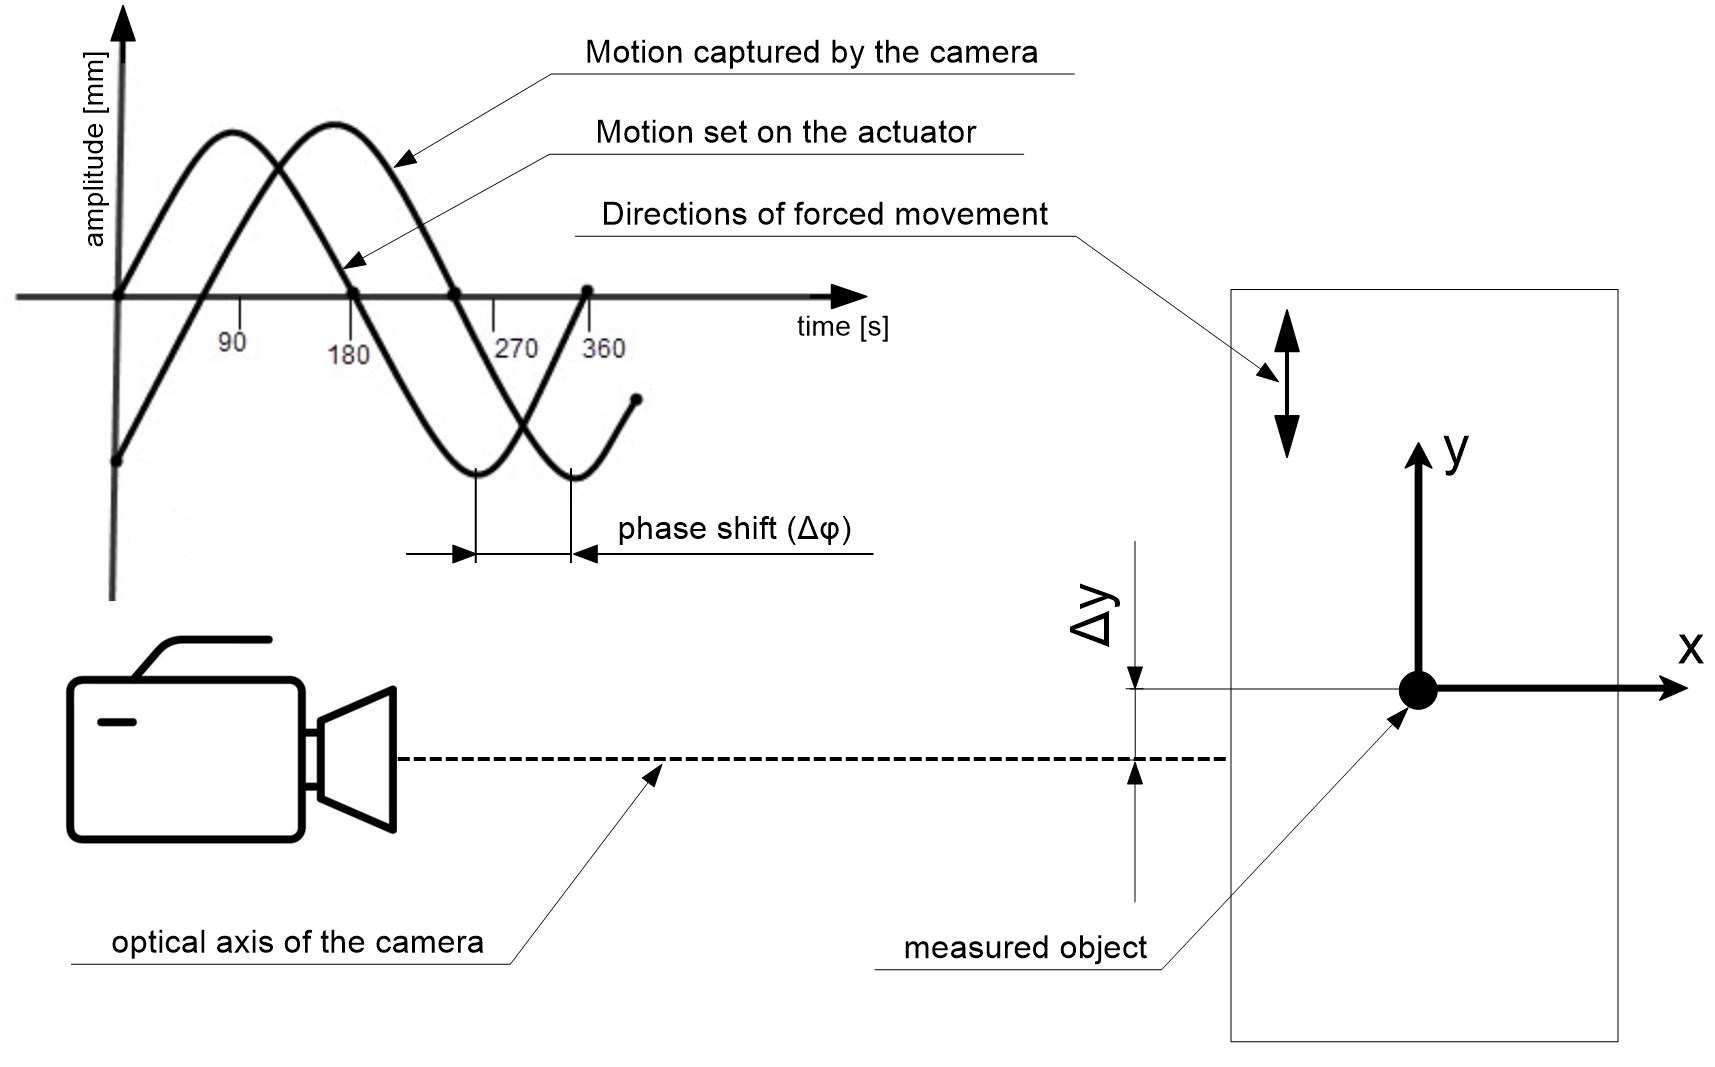
\includegraphics[width=0.9\textwidth]{../workspace/meas_problem.png} 
\end{center}
\caption{Idea problemu śledzenia obiektu na podstawie krzywej ruchu zadanej \\na siłowniku wymuszającym ruch.}
\label{fig:meas_problem}
\end{figure} 

\noindent W związku z powyższymi trudnościami zdecydowano się na rozwiązanie, w którym do układu pomiarowego wprowadzono dodatkowy obiekt.\\ \noindent Część drucika znajdująca się w polu widzenia kamery położona jest w jej płaszczyźnie ostrości. Dzięki takiemu zabiegowi zyskano dwie korzyści. Pierwsza z nich to brak zjawiska paralaksy pomiędzy badanym obiektem a obiektem referencyjnym. Druga to eliminacja potencjalnego błędu odwzorowania obrazu wynikająca z braku ostrości obiektu na rejestrowanych zdjęciach. Scenę z położeniem obiektu referencyjnego i kropli przedstawiono na rysunku \ref{fig:reference_img}:
\vspace{2mm}

\captionsetup{skip=0pt}
\begin{figure}[!h]
\captionsetup{justification=centering}
\begin{center}
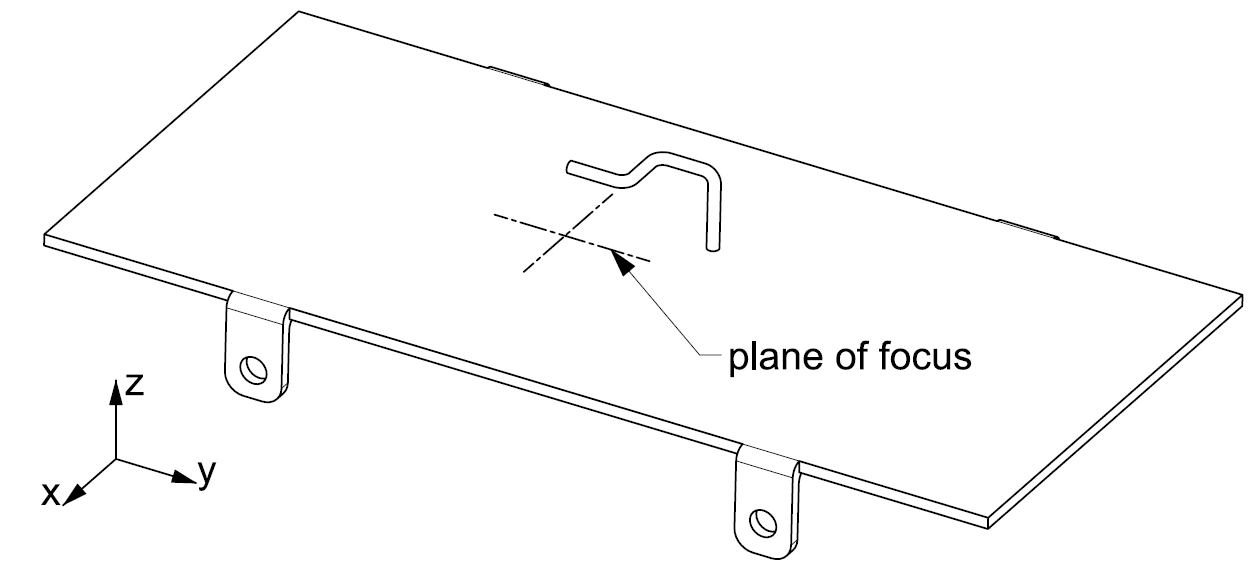
\includegraphics[width=1\textwidth]{../workspace/reference_object.png} 
\end{center}
\caption{Obiekt referencyjny służący do stabilizacji obrazu.}
\label{fig:reference_object}
\end{figure} 

\newpage
\captionsetup{skip=0pt}
 \begin{centering}
\begin{minipage}{0.5\textwidth}
\begin{figure}[H]
\captionsetup{justification=centering}
\begin{center}
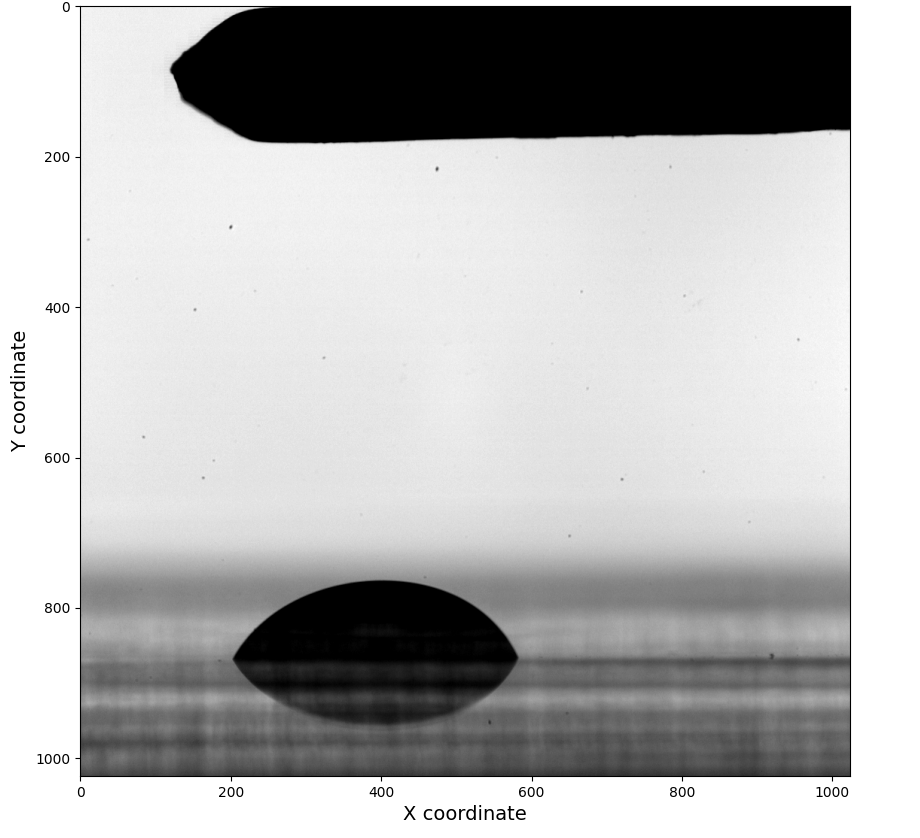
\includegraphics[width=1\textwidth]{../workspace/reference_img.png} 
\end{center}
\caption{\footnotesize Surowe dane pomiarowe. \\Obiekt referencyjny do stabilizacji obrazu.}
\label{fig:reference_img}
\end{figure}
\end{minipage}
  \begin{minipage}{0.5\textwidth}
\begin{figure}[H]
\captionsetup{justification=centering}
\begin{center}
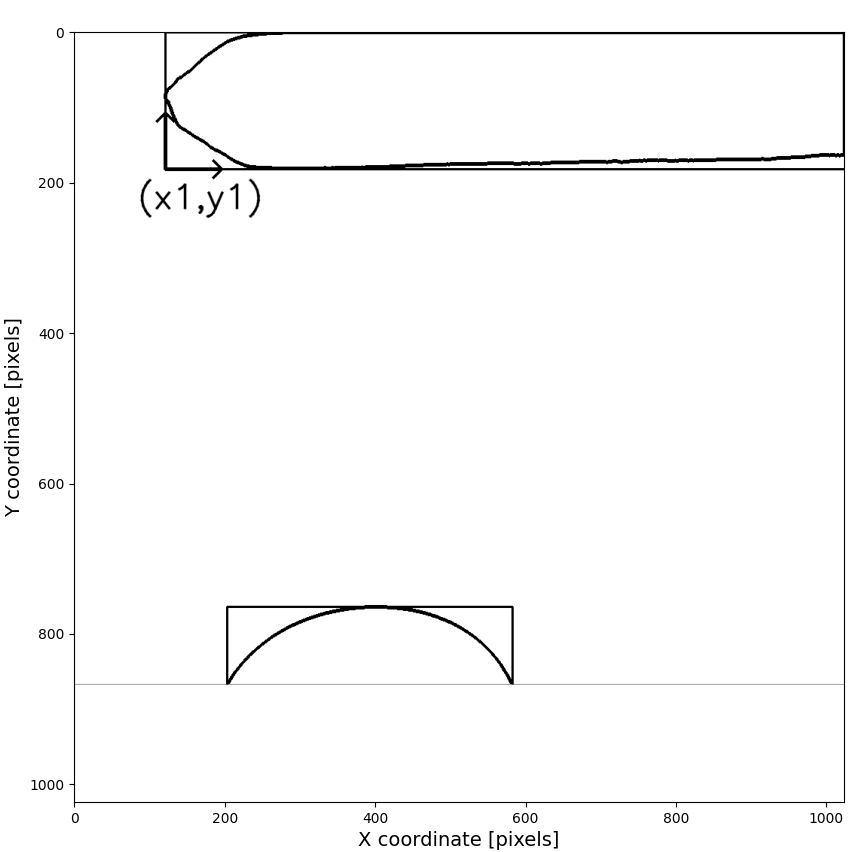
\includegraphics[width=0.95\textwidth]{../workspace/reference_binary.png} 
\end{center}
\caption{\footnotesize Sposób wyznaczenia układu współrzędnych stanowiącego punkt odniesienia do stabilizacji obrazu. Zastosowanie funkcji cv2.boundingRect().}
\label{fig:reference_binary}
\end{figure}
\end{minipage} \hfill
\end{centering}
\normalsize

\vspace{5mm}
\noindent Do detekcji konturu drucika użyto dokładnie tej samej metody, co w przypadku kropli (rozdz. \ref{chapter:contour_detection}). Wokół znalezionego konturu rozpięto kwadrat, który wyznaczony został przy pomocy funkcji \\cv2.boundingRect(). Funkcja ta służy do rysowania przybliżonego prostokąta wokół obrazu binarnego. Używana jest głównie do podświetlania obszaru zainteresowania po uzyskaniu konturów z obrazu, natomiast w naszym przypadku funkcja służy do wyznaczania ROI (\textit{ang. Region of Interest}) obiektu referencyjnego. W ten sposób można wyznaczyć położenie układu współrzędnych \textbf{(x1, y1)} (rys. \ref{fig:reference_binary}) na stałe związanego z ruchomą płytką. Umożliwi to śledzenie kropli w taki sposób, aby pozostawała ona ''nieruchoma'' na obrazie, zaś ruszać się będzie jedynie tło.

\subsection{Wyznaczanie kątów zwilżenia}
\noindent W tym podrozdziale opisano metodę pomiaru kątów zwilżenia. Dysponując obrazami w postaci binarnej proces obrabiania konturów sprowadza się do pracy w zakresie zbiorów dyskretnych, reprezentujących poszczególne piksele na obrazie. Ogólna koncepcja wyznaczenia kątów zwilżenia polega na interpolacji kształtu konturu za pomocą wielomianów rozpiętych na punktach pomiarowych (pikselach). Następnie w punktach pomiaru kątów zwilżenia wyznaczone zostaną styczne, na podstawie których obliczone zostaną współczynniki kierunkowe prostych. Ze względu na stabilność metody interpolacyjnej aproksymowane są jedynie fragmenty konturu tuż przy strefie kontaktu w płytką. \\
\noindent Do interpolacji kształtu kropli zastosowano funkcję \textit{polyfit()} dostępną w bibliotece \textbf{numpy}. Funkcja ta dopasowuje wielomian w postaci:
$$p(x) = p[0] \cdot x^{n} + p[1] \cdot x^{n-1} + ... + p[n]$$
\noindent do zbioru punktów (x,y), gdzie \textit{n} to stopień wielomianu interpolacyjnego zadany przez użytkownika. Rozwiązanie minimalizuje błąd kwadratowy zgodnie z formułą:
$$E = \sum_{j=0}^{k} |p(x_j) - y_j|^2$$
\newpage
\noindent dla układu równań w postaci:
$$x[0]^n \cdot p[0] +  x[0]^{n-1} \cdot p[1] + ... + x[0]\cdot p[n-1] + p[n] = y[0]$$
$$x[1]^n \cdot p[0] +  x[1]^{n-1} \cdot p[1] + ... + x[1]\cdot p[n-1] + p[n] = y[1]$$
$$...$$
$$x[k]^n \cdot p[0] +  x[k]^{n-1} \cdot p[1] + ... + x[k]\cdot p[n-1] + p[n] = y[k]$$
\noindent gdzie k to liczba punktów pomiarowych.\\
\noindent Macierz współczynników wektora \textbf{p} jest macierzą Vandermonde'a \cite{ALGEBRA}.\\\\

\noindent Nasuwa się zatem pytanie, jaki wpływ na dokładność interpolacji ma w ogólnym przypadku stopień wielomianu. W celu weryfikacji tej zależności przeprowadzono dwie analizy, w których stopień wielomianu ustawiono odpowiednio jako 2 i 5. Jak wspomniano wcześniej, interpolacji nie podlega cały kontur, a jedynie obszary znajdujące się w pobliżu strefy kontaktu kropla - płytka. Obszar ten wydzielono poprzez wyselekcjonowanie zbioru punktów poniżej zadanej prostej geometrycznej. W wyniku tego, w procesie interpolacji bierze udział pewien podzbiór punktów. Ilość punktów jest wystarczająca do dobrego odwzorowania krzywej. Wyniki przedstawiono w formie wizualnej (rys. \ref{fig:polynomial_fit_2deg} - rys. \ref{fig:polynomial_fit_5deg}), zestawiając ze sobą wykresy przedstawiające kontur i jego częściową interpolację w kolejnych chwilach czasowych (kolejnych klatkach). Szczególnie istotne są klatki, w których kształt kropli ''przegina się'' przeciwnie do kierunku ruchu (efekt bezwładności). 

\captionsetup{skip=0pt}
\begin{figure}[!h]
\captionsetup{justification=centering}
\begin{center}
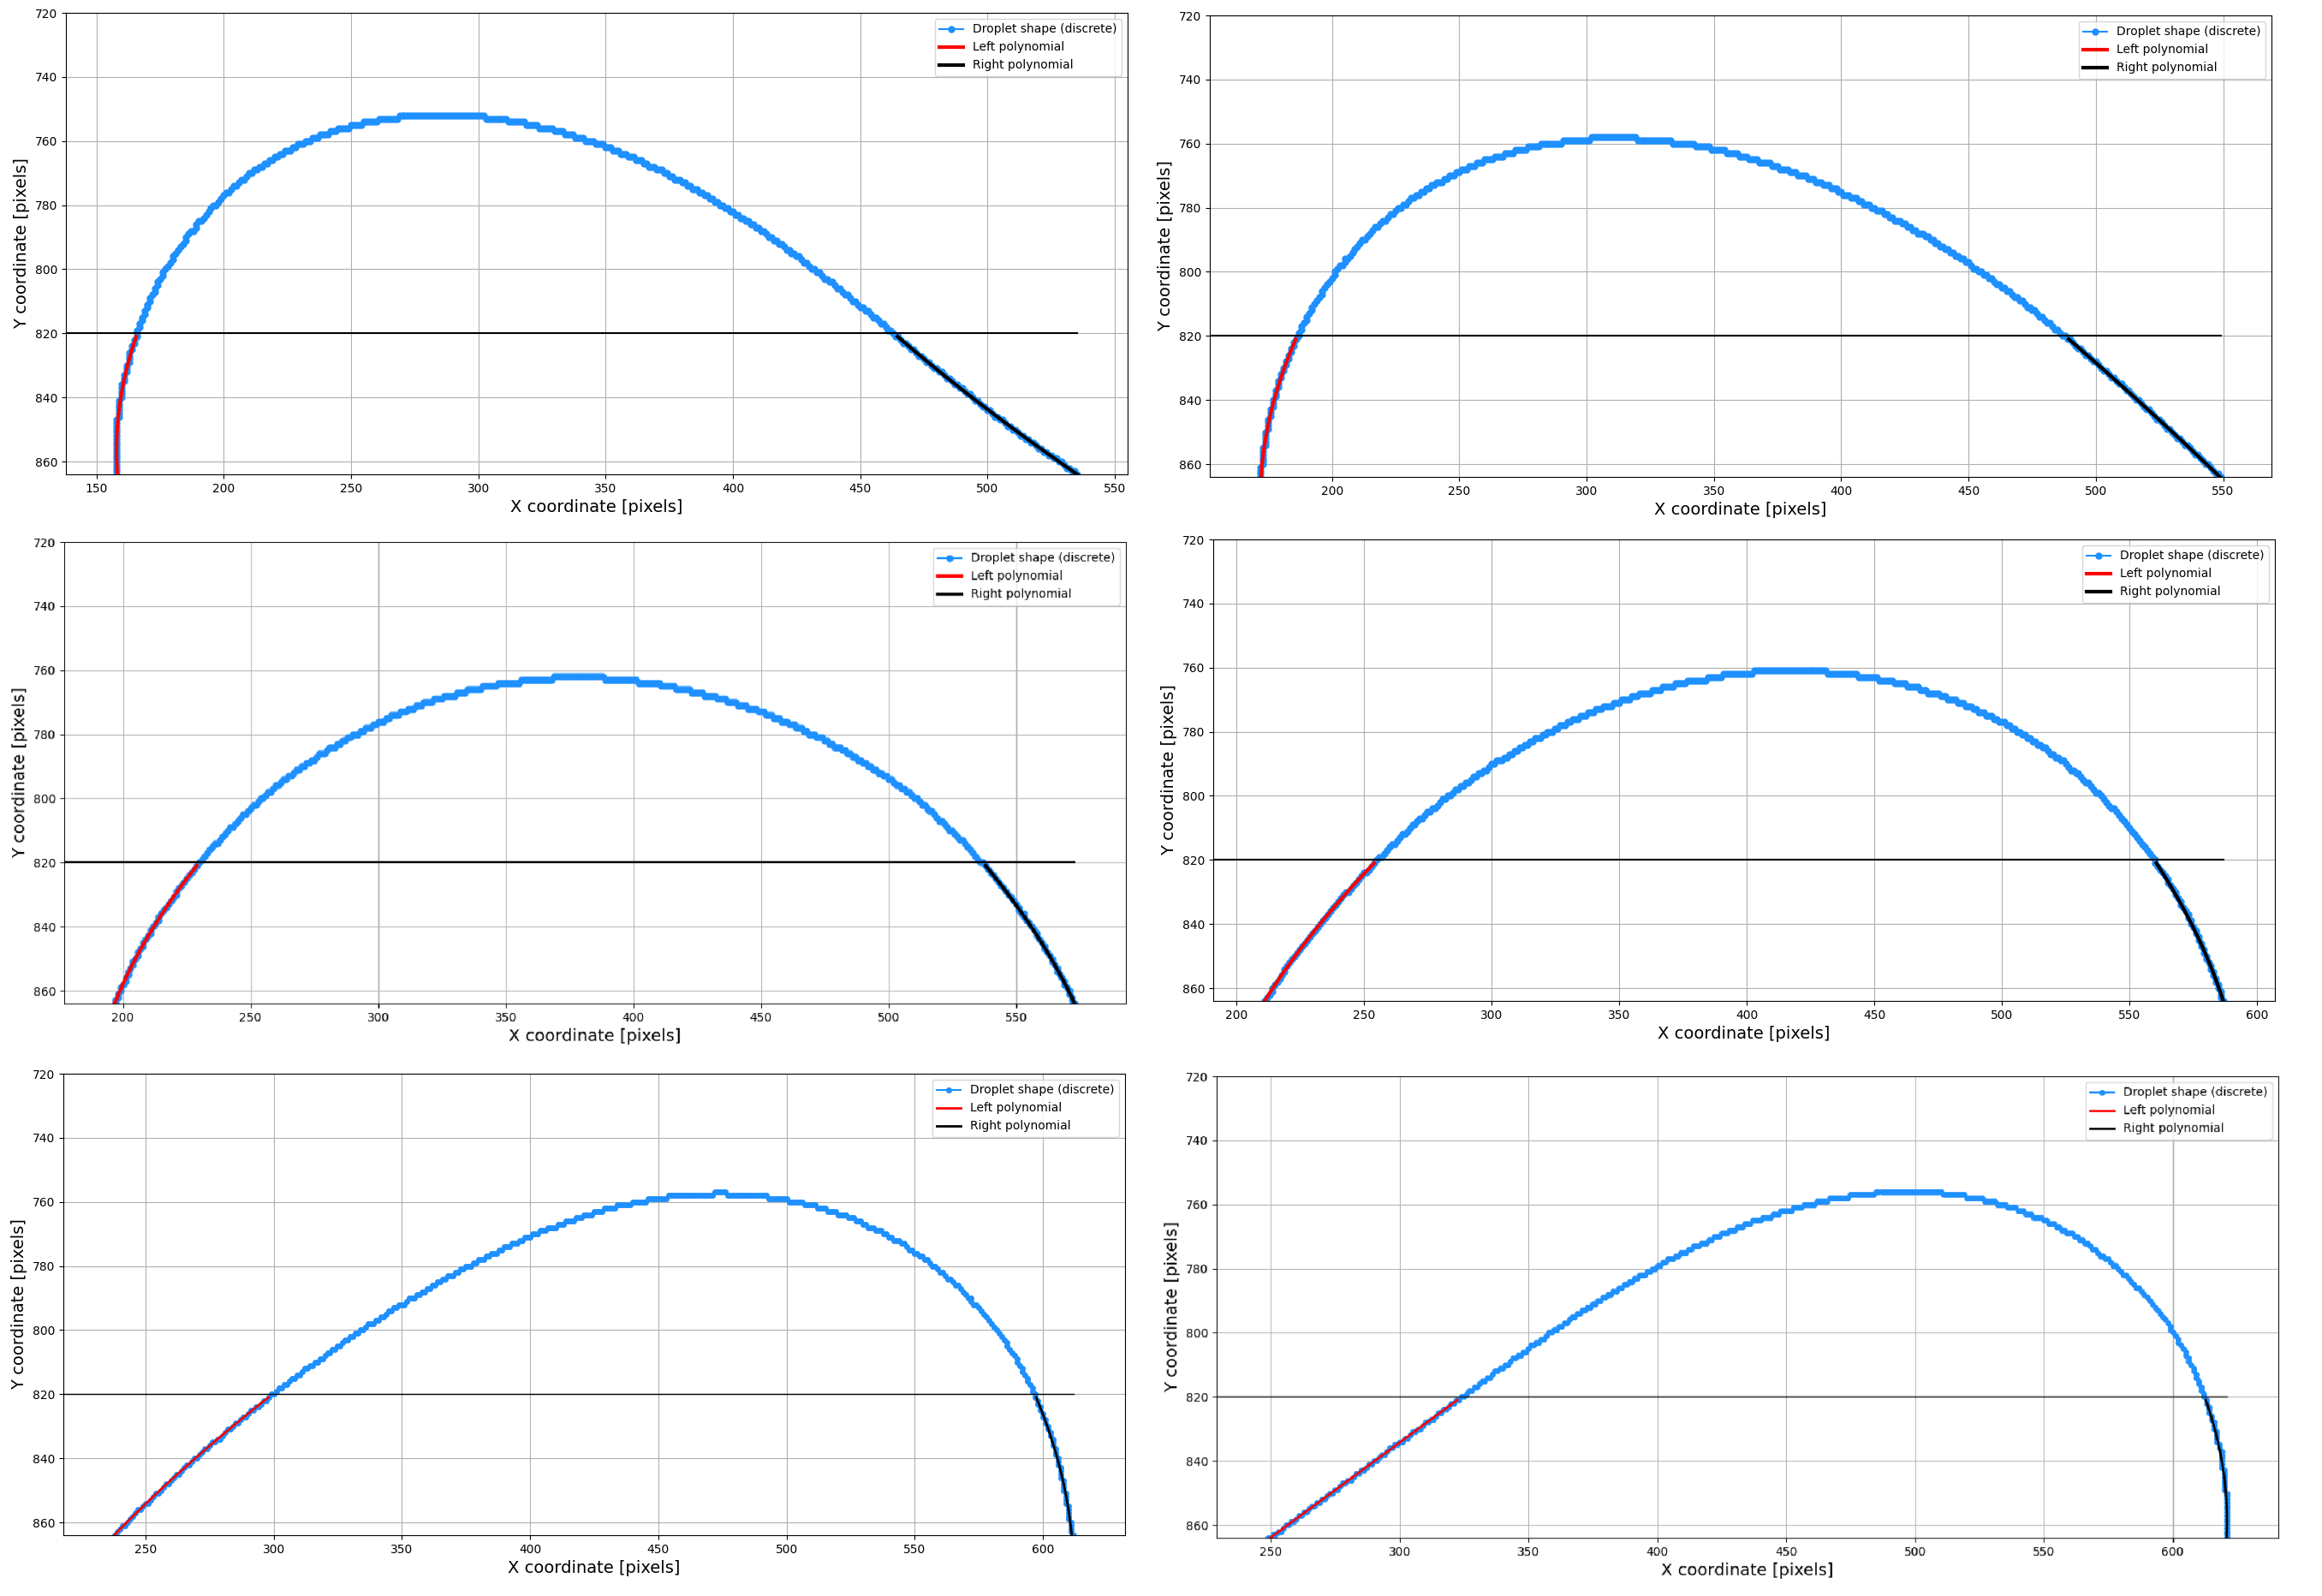
\includegraphics[width=1\textwidth]{../workspace/polynominal_fit_2deg.png} 
\end{center}
\caption{Zestawienie konturów (kolor niebieski) i wielomianów interpolowanych na określonych przedziałach dla kolejnych chwil czasowych (klatek). \textbf{Stopień wielomianów interpolacyjnych: 2}}
\label{fig:polynomial_fit_2deg}
\end{figure} 
\newpage


\captionsetup{skip=0pt}
\begin{figure}[!h]
\captionsetup{justification=centering}
\begin{center}
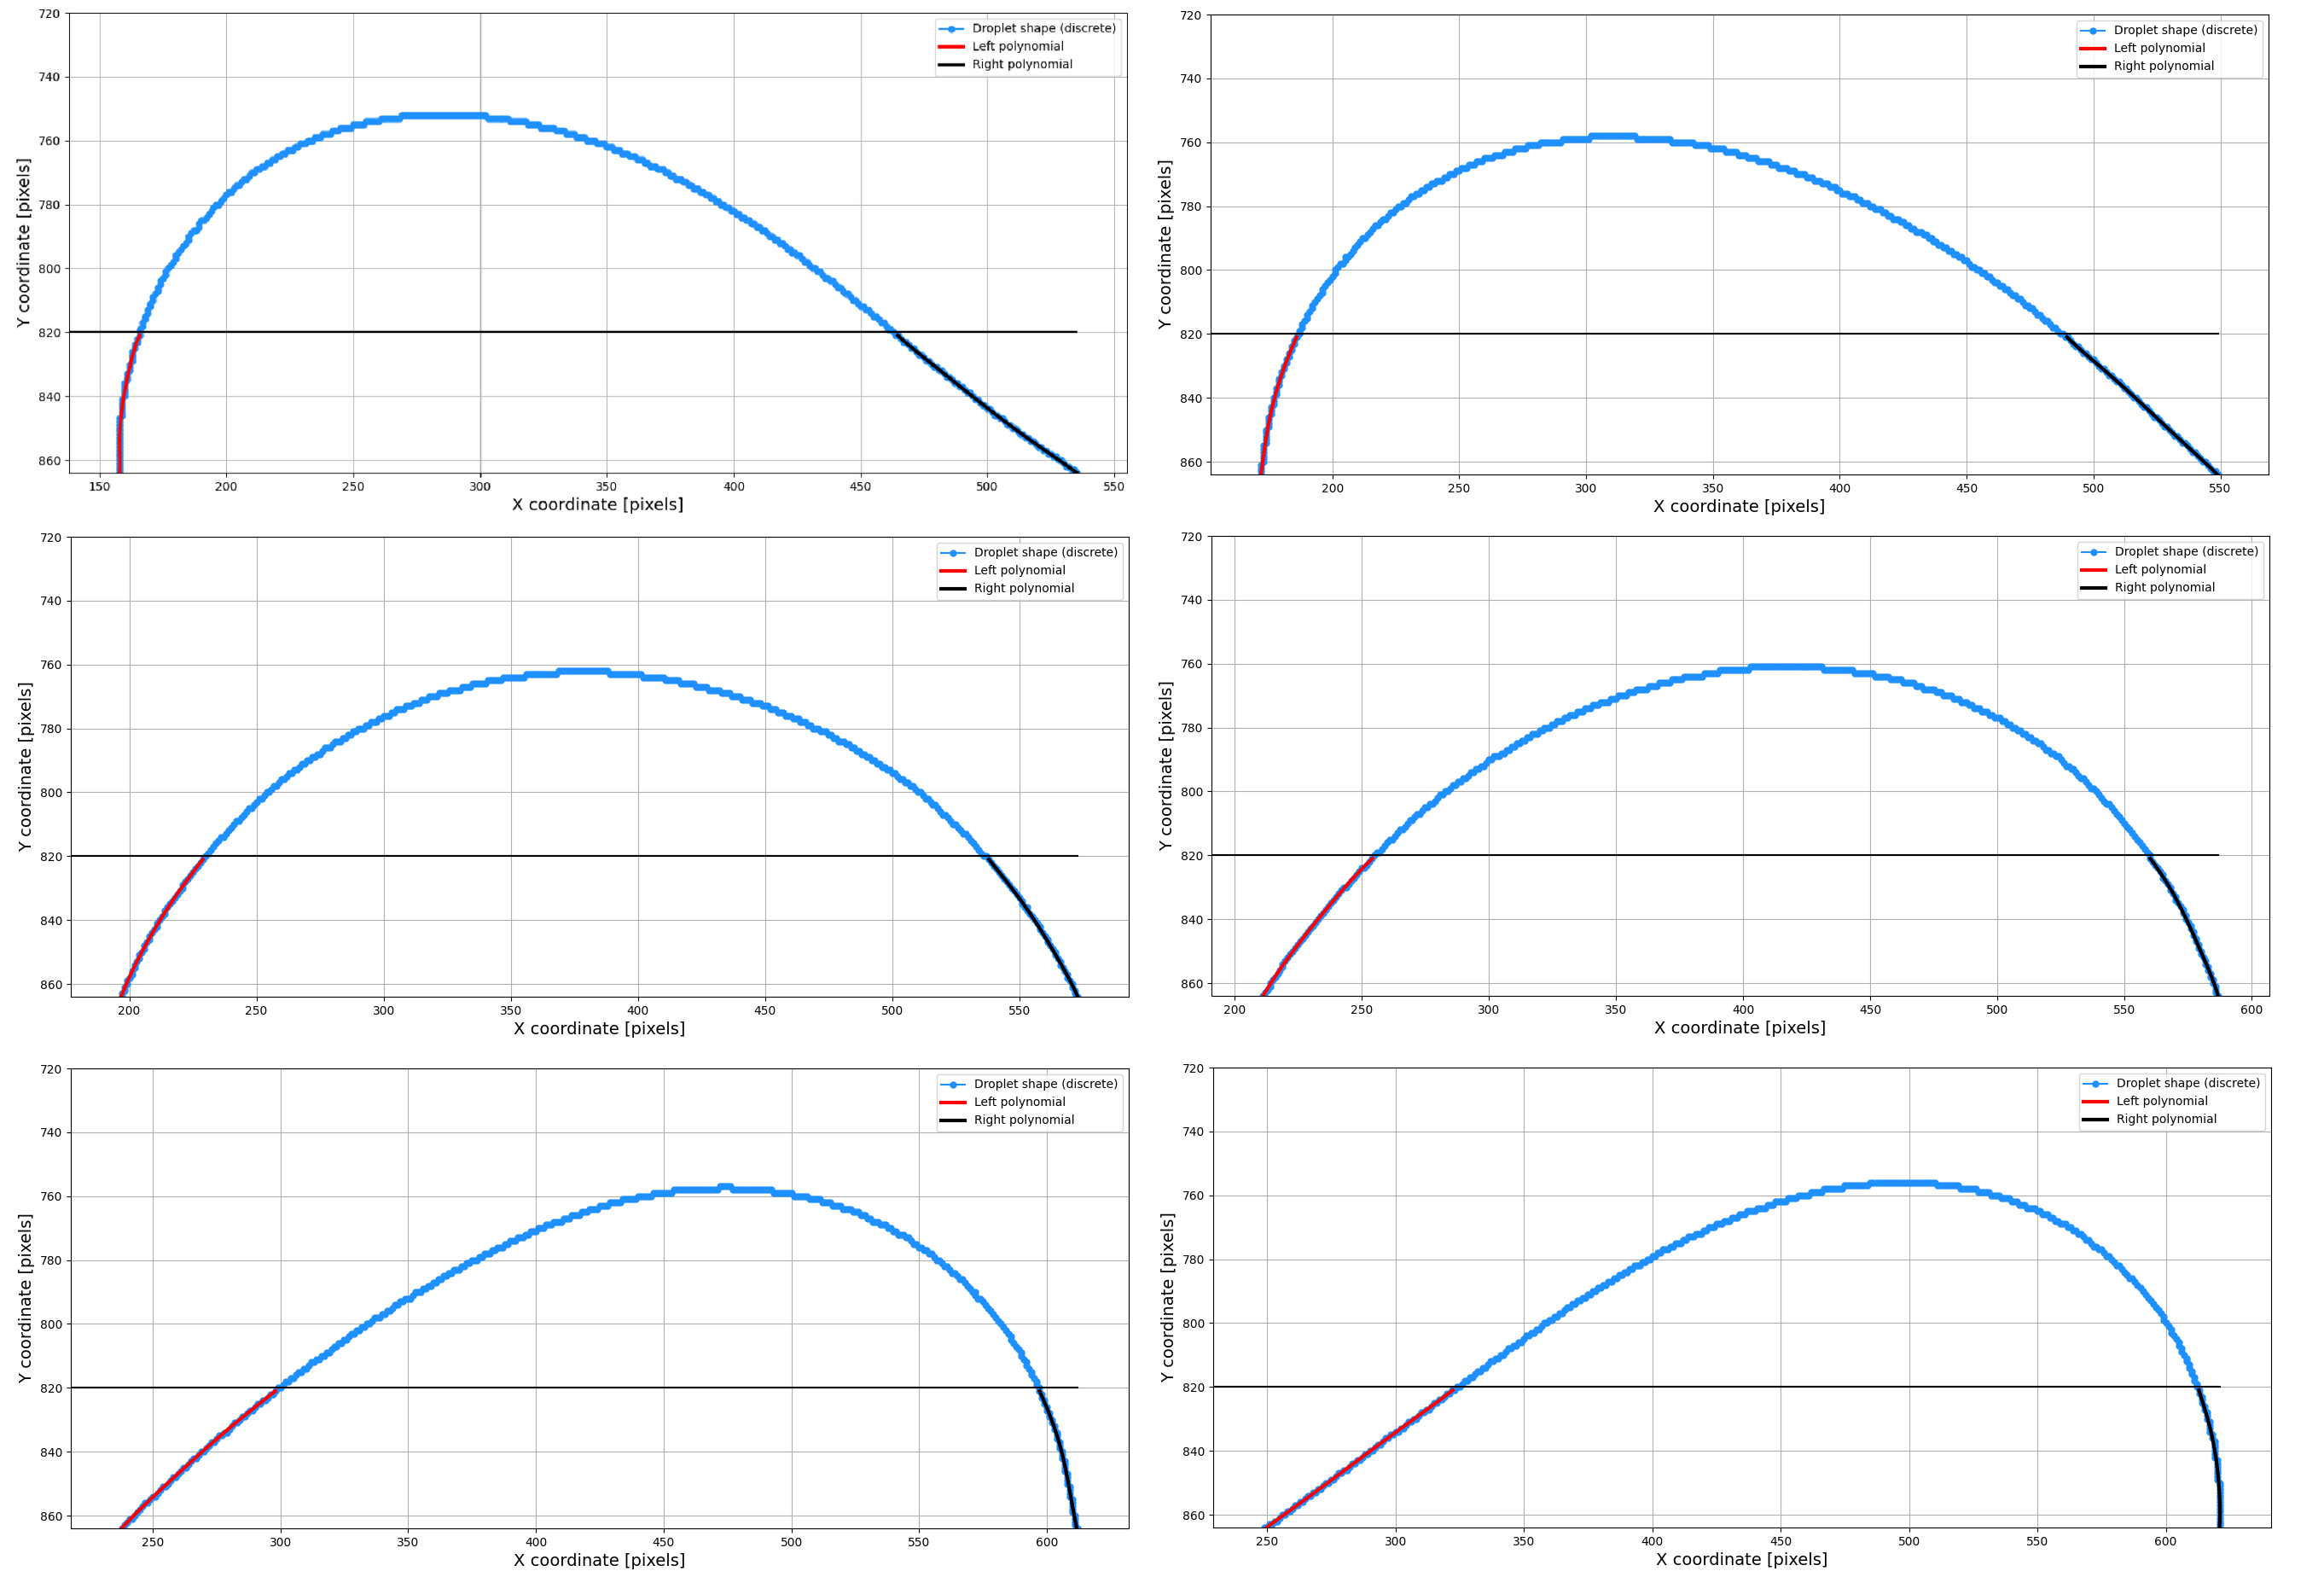
\includegraphics[width=0.95\textwidth]{../workspace/polynominal_fit_5deg.png} 
\end{center}
\caption{Zestawienie konturów (kolor niebieski) i wielomianów interpolowanych na określonych przedziałach dla kolejnych chwil czasowych (klatek). \textbf{Stopień wielomianów interpolacyjnych: 5}}
\label{fig:polynomial_fit_5deg}
\end{figure} 

\noindent Przedstawione wykresy wskazują na to, że interpolacja za pomocą wielomianu o stopniu zarówno 2, jak i 5 dobrze odwzorowuje kontur kropli. Różnice pomiędzy przedstawionymi danymi nie są widoczne gołym okiem. W celu porównania metod zbadano przebieg przyrostu kąta w kolejnych klatkach zdefiniowany jako ($\theta_{i+1} - \theta_{i}$). Tak zdefiniowany parametr jest dobrym wskaźnikiem stabilności metody. Im przebieg ten jest bardziej gładki, tym metoda charakteryzuje się mniejszym błędem numerycznym. Analizę tę przeprowadzono w krótkim okresie czasu.

\captionsetup{skip=0pt}
\begin{figure}[!h]
\captionsetup{justification=centering}
\begin{center}
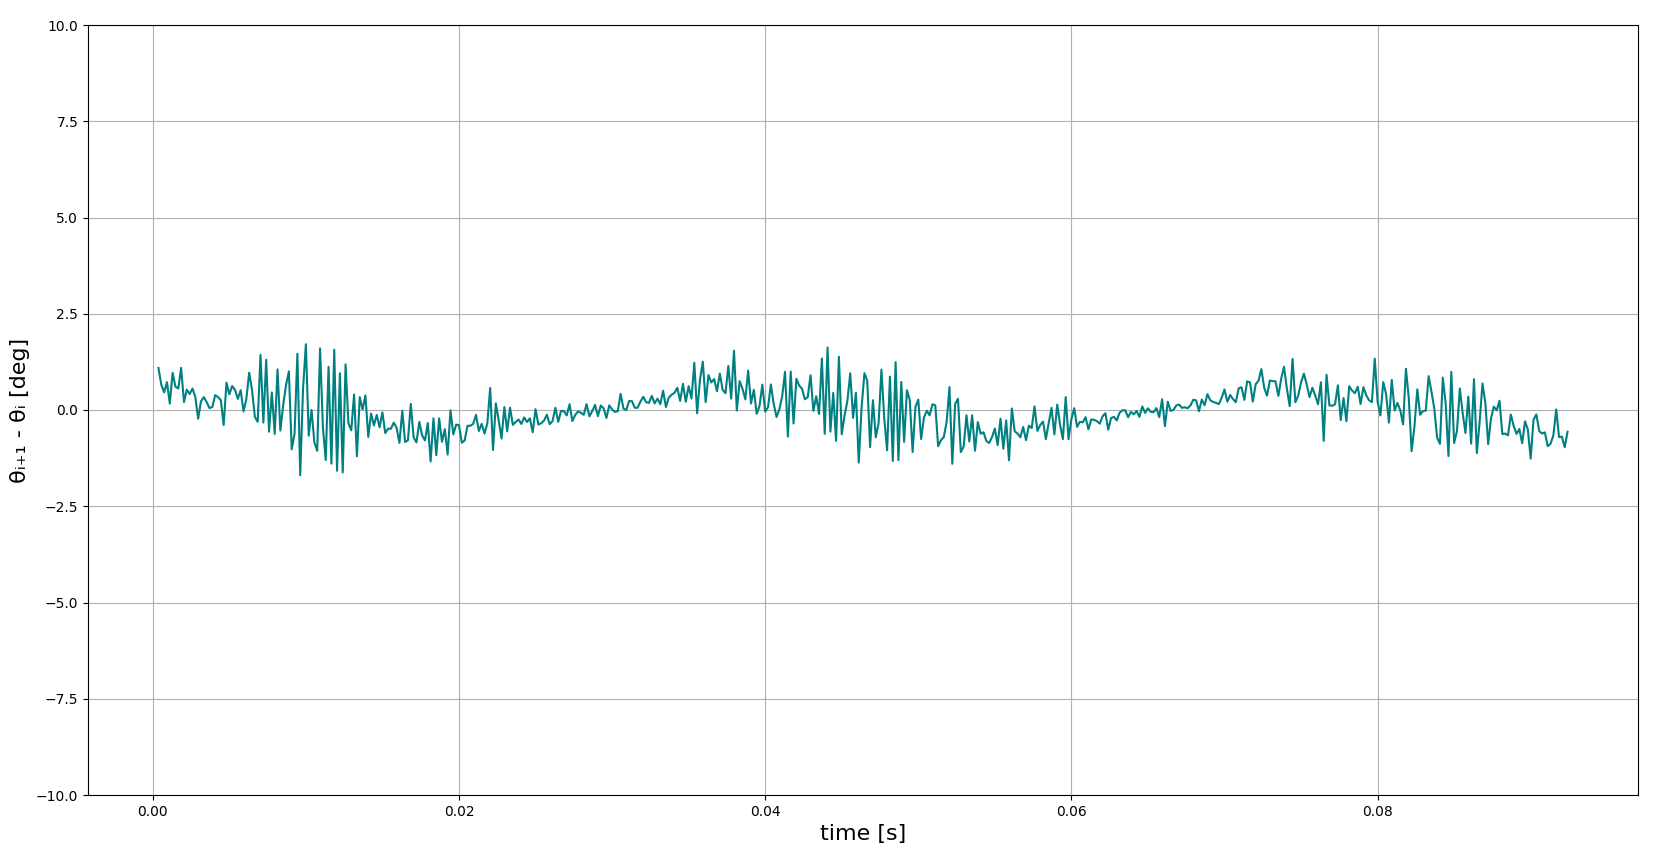
\includegraphics[width=0.85\textwidth]{../workspace/deg2_diff.png} 
\end{center}
\caption{Przebieg przyrostu kąta ($\theta_{i+1} - \theta_{i}$) w kolejnych chwilach czasowych. \\Indeks (i+1) oznacza kolejną klatkę nagrania.  \textbf{Stopień wielomianów interpolacyjnych: 2}}
\label{fig:deg2_diff}
\end{figure} 
\newpage

\noindent Pomiar ten powtórzono z zastosowaniem stopnia wielomianu interpolacyjnego równego 5 (rys. \ref{fig:deg5_diff}). Wynik zaskakująco dobrze pokazuje, że zwiększanie stopnia wielomianu powoduje utratę stabilności metody, tzn. wzrasta błąd związany z pomiarem kąta 
\captionsetup{skip=0pt}
\begin{figure}[!h]
\captionsetup{justification=centering}
\begin{center}
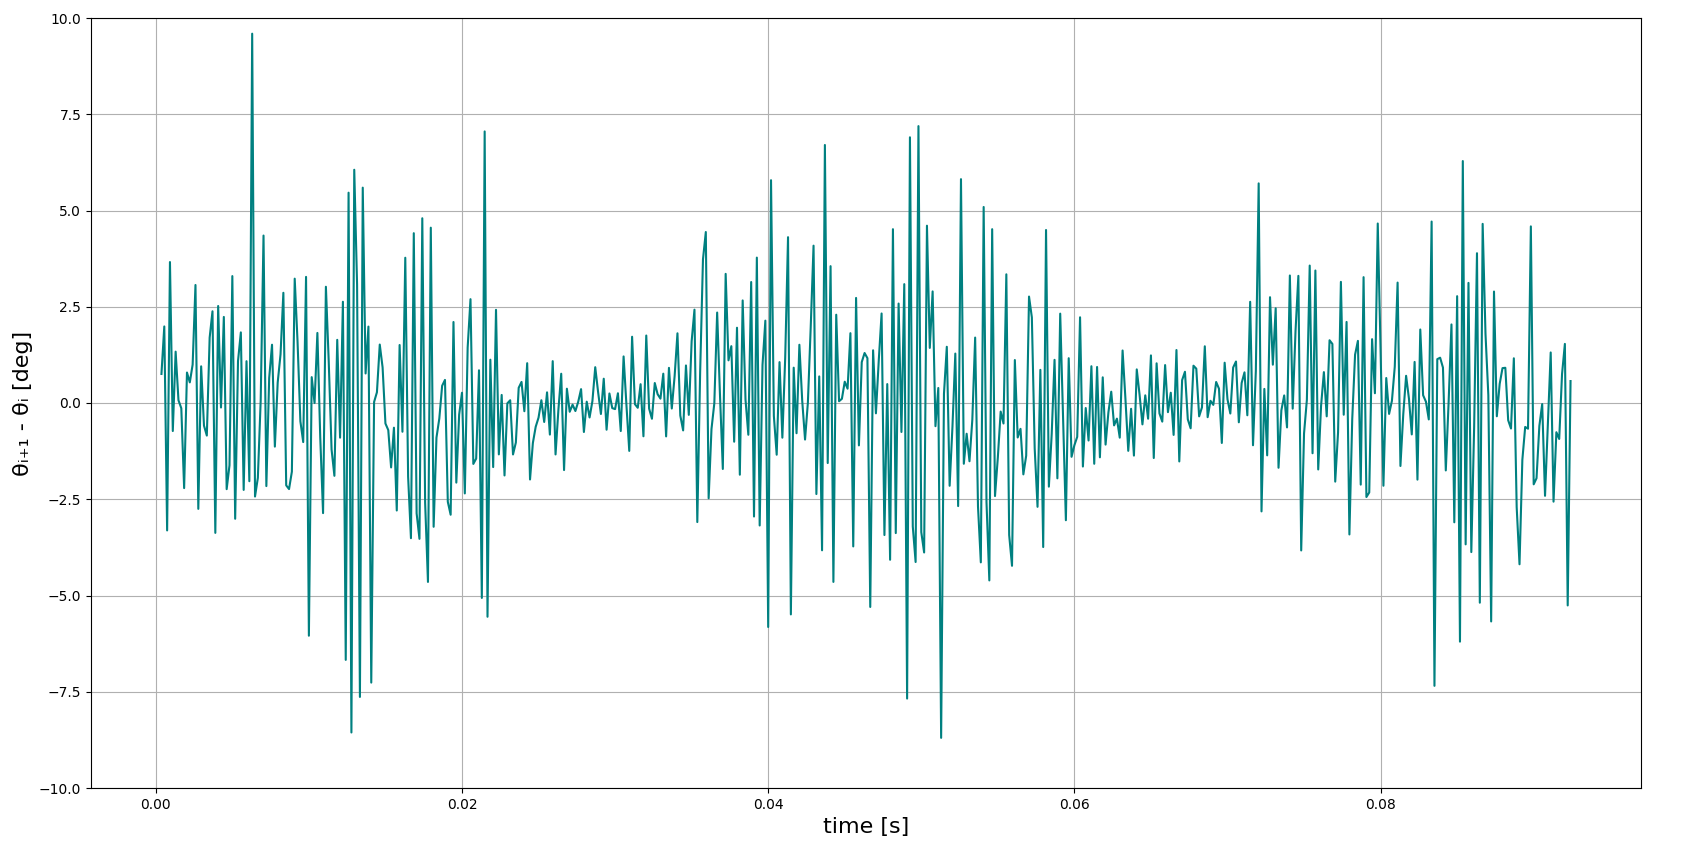
\includegraphics[width=0.85\textwidth]{../workspace/deg5_diff.png} 
\end{center}
\caption{Przebieg przyrostu kąta ($\theta_{i+1} - \theta_{i}$) w kolejnych chwilach czasowych. \\Indeks (i+1) oznacza kolejną klatkę nagrania.  \textbf{Stopień wielomianów interpolacyjnych: 5}}
\label{fig:deg5_diff}
\end{figure} 


\noindent Mając na uwadze powyższe dane, do pomiaru kąta zastosowano wielomian niskiego rzędu (2). Dane pomiarowe zapisywano do plików w formacie CSV. Strukturę danych w plikach przedstawiono w poniższej tabeli:

\captionsetup{skip=2pt}
\begin{table}[h!]
\captionsetup{justification=centering}
\caption{Struktura plików CSV przechowujących dane pomiarowe.}
\begin{tabular}{| p{0.10\linewidth}| p{0.15\linewidth} | p{0.20\linewidth} | p{0.20\linewidth} | p{0.20\linewidth} |}
\hline
Nazwa kolumny & Col0  & Col1  & Col2  & Col3  \\ \hline
Typ  & Czas [s]  & Kąt zwilżania (lewy) [deg]  & Kąt zwilżania (prawy) [deg]  & Długość strefy kontaktu [px] \\ \hline
Format & float64 & float64 & float64 & int64 \\ \hline
\end{tabular}
\end{table}

\vspace{8mm}
\noindent Na poniższym diagramie przedstawiono schematycznie proces przetwarzania danych. W następnych krokach dane poddane zostaną transformacji Fouriera.
\captionsetup{skip=0pt}
\begin{figure}[!h]
\captionsetup{justification=centering}
\begin{center}
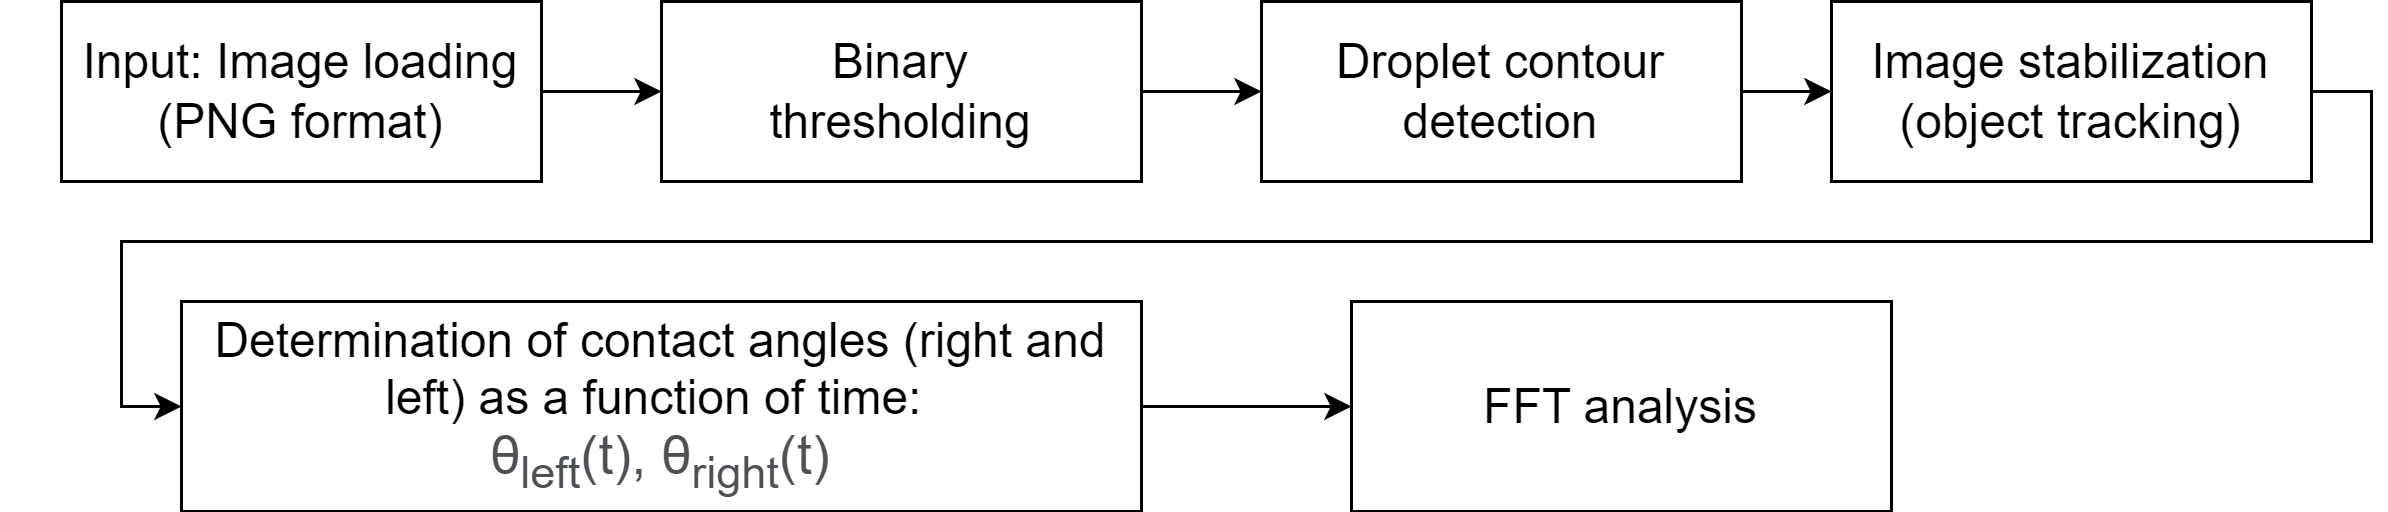
\includegraphics[width=1\textwidth]{../workspace/workflow.png} 
\end{center}
\caption{Struktura programu i kolejność wykonywanych operacji.}
\label{fig:deg5_diff}
\end{figure} 



\newpage
\noindent Kilka przykładowych klatek nagrania, które zostały w pełni przetworzone przedstawiono na poniższych rysunkach. Reprezentują one wynik końcowy obróbki zdjęć. 

\captionsetup{skip=0pt}
 \begin{centering}
\begin{minipage}{0.5\textwidth}
\begin{figure}[H]
\captionsetup{justification=centering}
\begin{center}
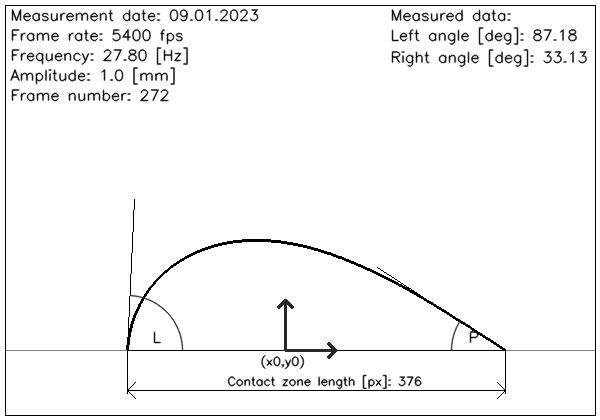
\includegraphics[width=1\textwidth]{../workspace/conv_img1.png} 
\end{center}
\end{figure}
\end{minipage}
  \begin{minipage}{0.5\textwidth}
\begin{figure}[H]
\captionsetup{justification=centering}
\begin{center}
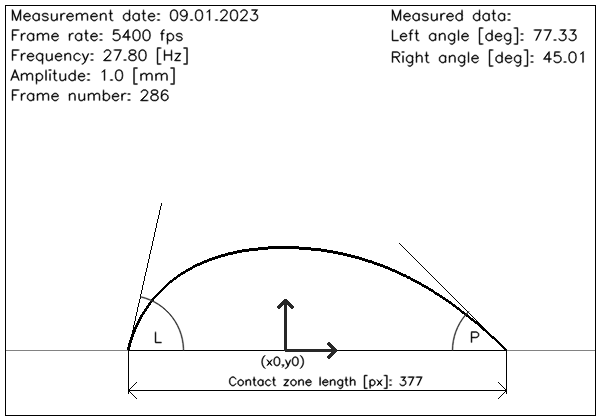
\includegraphics[width=1\textwidth]{../workspace/conv_img2.png} 
\end{center}
\end{figure}
\end{minipage} \hfill
\end{centering}


\captionsetup{skip=0pt}
 \begin{centering}
\begin{minipage}{0.5\textwidth}
\begin{figure}[H]
\captionsetup{justification=centering}
\begin{center}
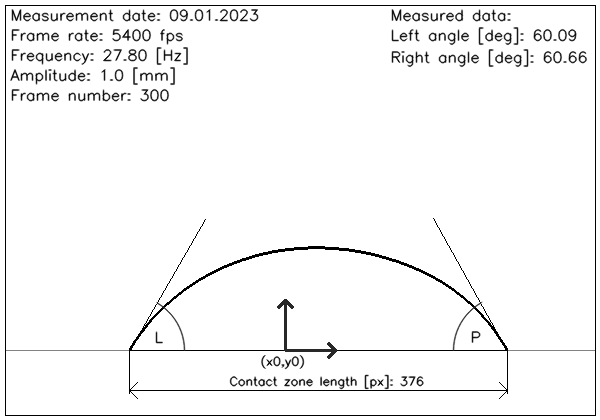
\includegraphics[width=1\textwidth]{../workspace/conv_img3.png} 
\end{center}
\end{figure}
\end{minipage}
  \begin{minipage}{0.5\textwidth}
\begin{figure}[H]
\captionsetup{justification=centering}
\begin{center}
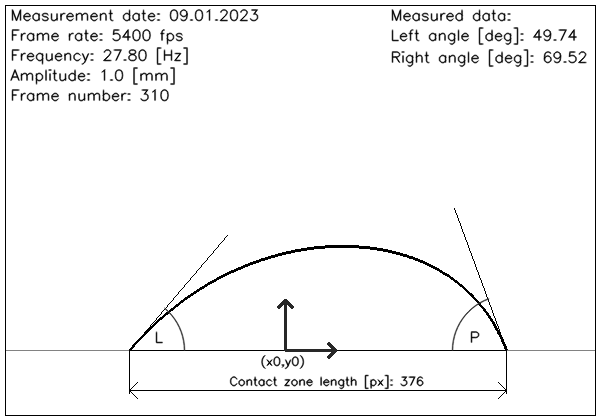
\includegraphics[width=1\textwidth]{../workspace/conv_img4.png} 
\end{center}
\end{figure}
\end{minipage} \hfill
\end{centering}


\captionsetup{skip=0pt}
 \begin{centering}
\begin{minipage}{0.5\textwidth}
\begin{figure}[H]
\captionsetup{justification=centering}
\begin{center}
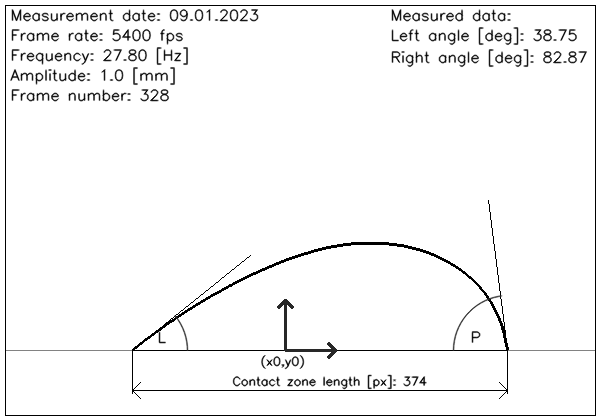
\includegraphics[width=1\textwidth]{../workspace/conv_img5.png} 
\end{center}
\end{figure}
\end{minipage}
  \begin{minipage}{0.5\textwidth}
\begin{figure}[H]
\captionsetup{justification=centering}
\begin{center}
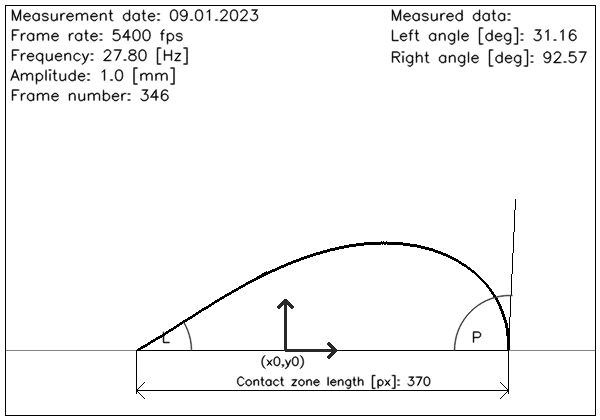
\includegraphics[width=1\textwidth]{../workspace/conv_img6.png} 
\end{center}
\end{figure}
\end{minipage} \hfill
\end{centering}
\newpage

\section{Pomiar kątów zwilżania - graficzna reprezentacja danych}
\noindent Dla każdego zestawu danych pomiarowych wygenerowano wykresy przedstawiające przebieg wartości kątów zwilżenia w funkcji czasu. Na wykresie zawarto także zmiany długości strefy kontaktu pomiędzy kroplą a platformą. Tak sporządzone wykresy stanowią jeden z pierwszych etapów weryfikacji poprawności pomiarów. Podczas analizy wykresów zauważono, że drgania kropli wywołują zmianę długości strefy kontaktu. Zmiana ta zależy od amplitudy i częstotliwości drgań, jednak sam efekt można opisać jako ''pełzanie''. Co więcej, przebieg wartości kątów zwilżenia dowodzi, że dla małych częstotliwości pojawiają się różne postacie drgań. \\

\noindent Charakterystyki dla mierzonych kątów (tj. kąta wyprzedzającego i podążającego) wykazują taką własność, że dla małej częstotliwości drgań wartość tych kątów różni się w zależności od kierunku ruchu. To znaczy, że w przypadku ruchu zgodnego z kierunkiem osi układu współrzędnych wartość kąta wyprzedzającego (\textit{ang. advancing angle}) jest większa niż w przypadku ruchu w kierunku przeciwnym. To samo można powiedzieć o kącie podążającym (\textit{ang. receding angle}). Efekt ten znany jest jako histereza kąta zwilżania i polega w ogólności na tym, że wartość kąta zwilżania cieczy postępującej po powierzchni ciała stałego przekracza wartość kąta zwilżania cieczy cofającej się na tej powierzchni. Na poniższych wykresach (rys. \ref{fig:theta(t)_1} - rys. \ref{fig:theta(t)_7}) przedstawiono charakterystyki otrzymane dla pomiarów o amplitudzie drgań równej 1 mm. Kolejność wykresów jest zgodna z narastającą częstotliwością drgań.


\captionsetup{skip=0pt}
\begin{figure}[!h]
\captionsetup{justification=centering}
\begin{center}
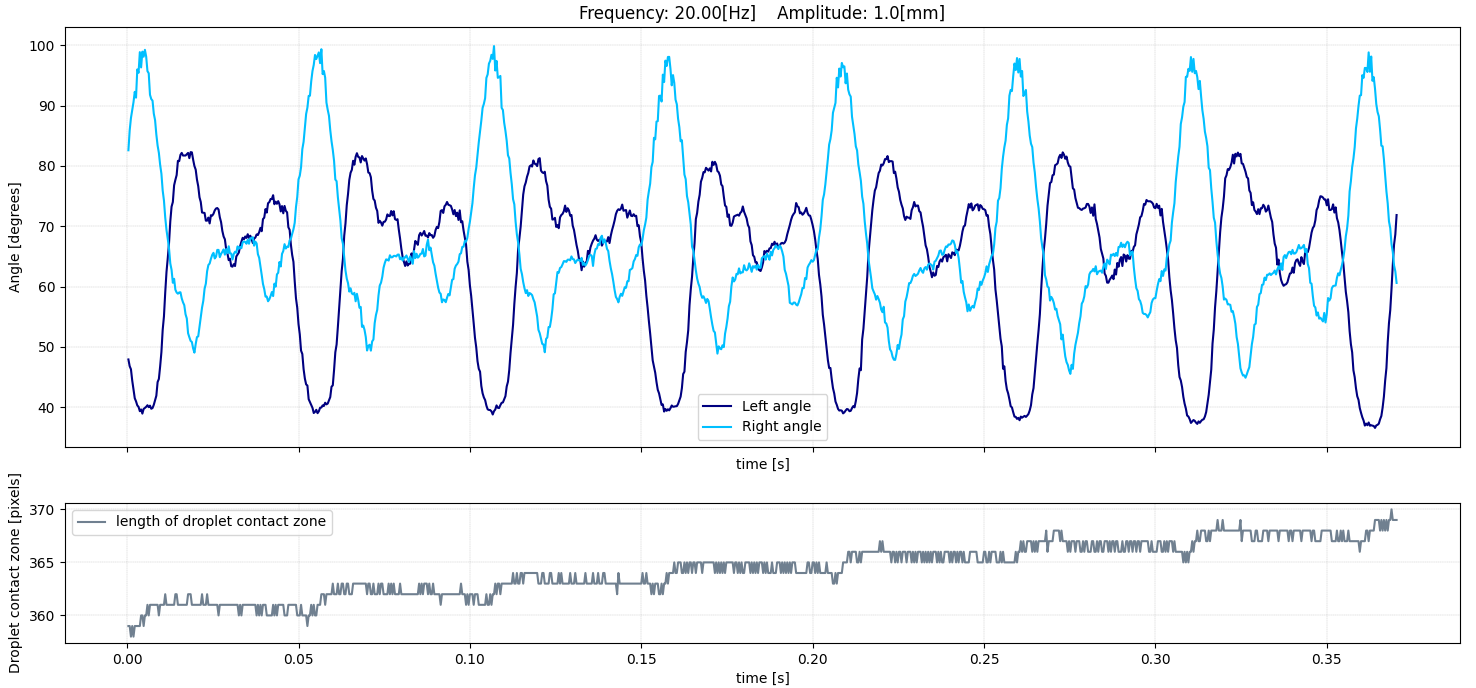
\includegraphics[width=1\textwidth]{../workspace/a10_f100z.png} 
\end{center}
\caption{Charakterystyka kątów zwilżania dla sinusoidalnego wymuszenia ruchu.  \\Amplituda drgań: 1.0 mm,  częstotliwość: 20 Hz.}
\label{fig:theta(t)_1}
\end{figure} 
\noindent Zjawisko nakładania się postaci drgań jest szczególnie widoczne na rys. \ref{fig:theta(t)_1} i zanika w miarę zwiększania częstotliwości (postać dominująca charakteryzuje się wtedy znacznie większą amplitudą). Warto dodać, że wykresy ilustrują przebieg pomiaru dla stosunkowo krótkiego czasu. Dla większych przedziałów czasu nie zauważono zmian przebiegu kątów zwilżenia. Zmiany te natomiast obejmują długość strefy kontaktu, która jak widać na powyższym wykresie, narasta.


\newpage
\captionsetup{skip=0pt}
\begin{figure}[!h]
\captionsetup{justification=centering}
\begin{center}
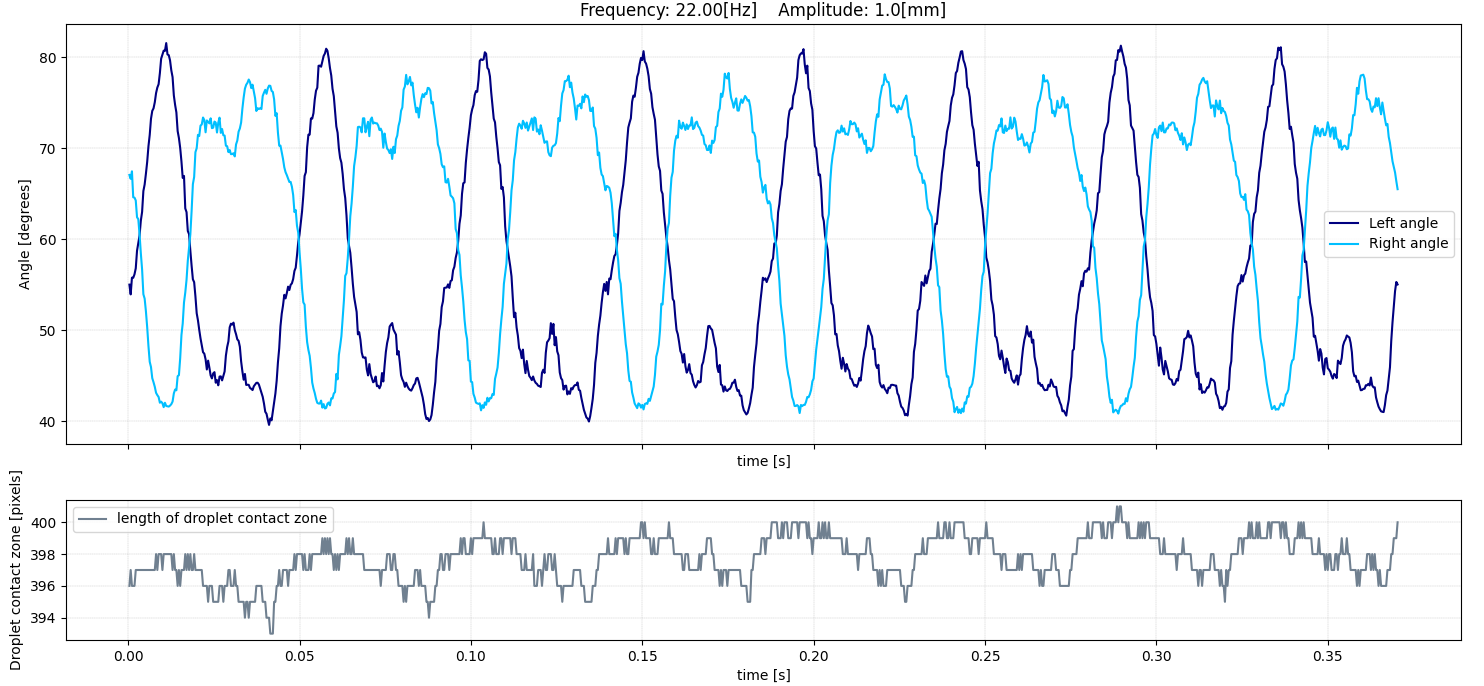
\includegraphics[width=1\textwidth]{../workspace/a10_f110z.png} 
\end{center}
\caption{Charakterystyka kątów zwilżania dla sinusoidalnego wymuszenia ruchu.  \\Amplituda drgań: 1.0 mm,  częstotliwość: 22 Hz.}
\label{fig:theta(t)_2}
\end{figure} 

\captionsetup{skip=0pt}
\begin{figure}[!h]
\captionsetup{justification=centering}
\begin{center}
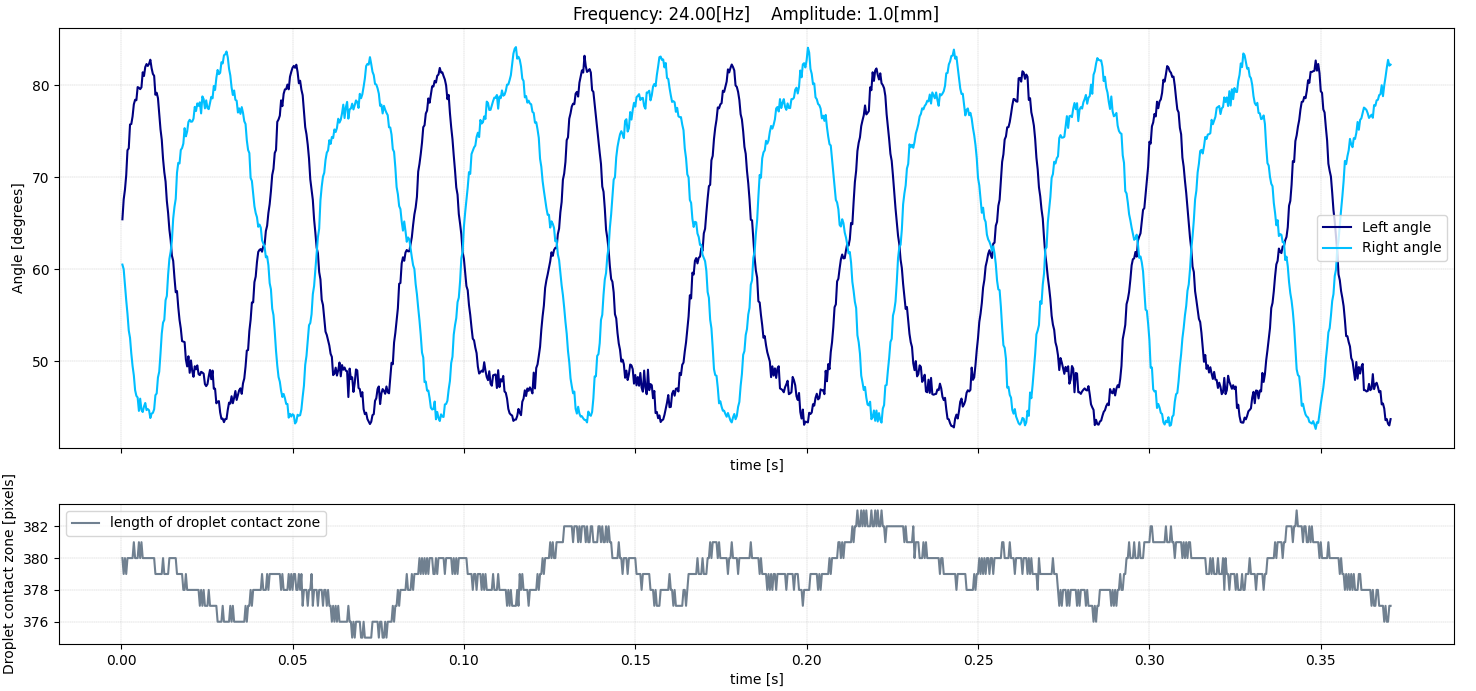
\includegraphics[width=1\textwidth]{../workspace/a10_f120z.png} 
\end{center}
\caption{Charakterystyka kątów zwilżania dla sinusoidalnego wymuszenia ruchu.  \\Amplituda drgań: 1.0 mm,  częstotliwość: 24 Hz.}
\label{fig:theta(t)_3}
\end{figure} 
\newpage

\captionsetup{skip=0pt}
\begin{figure}[!h]
\captionsetup{justification=centering}
\begin{center}
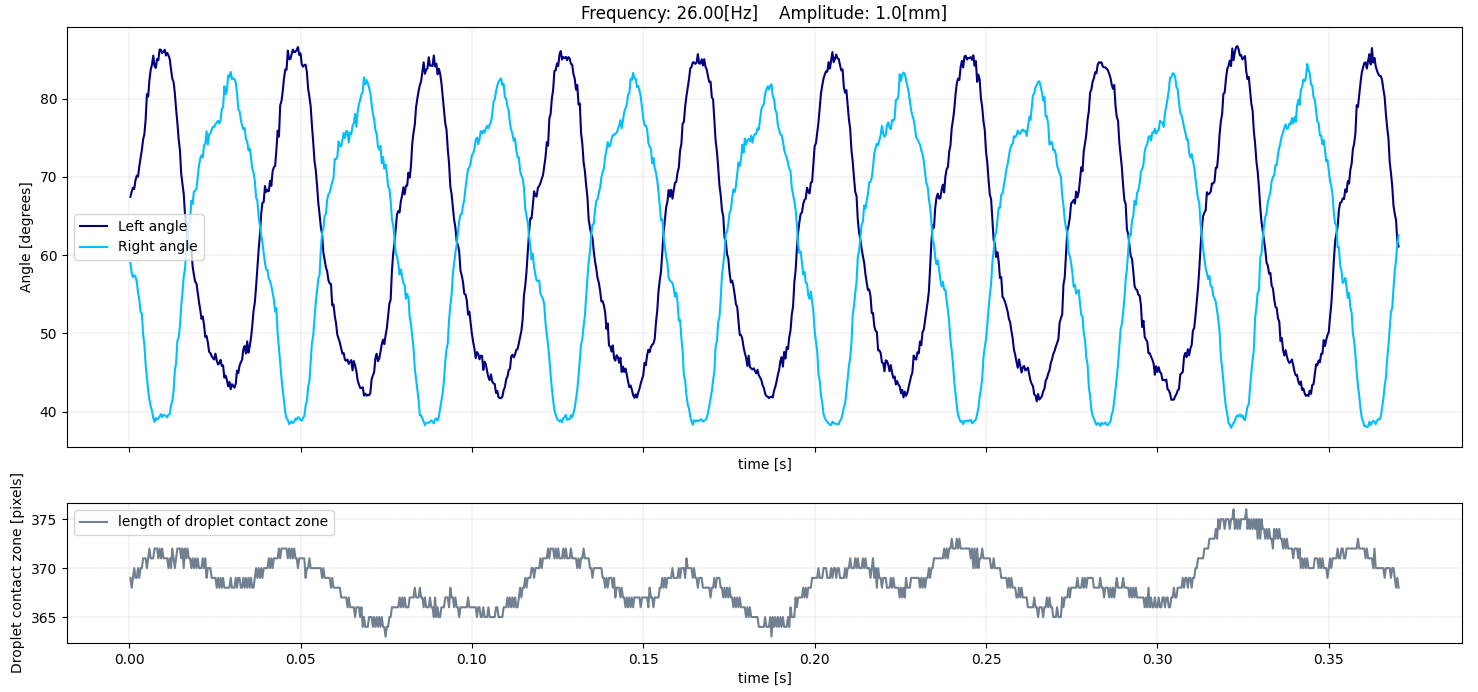
\includegraphics[width=1\textwidth]{../workspace/a10_f130z.png} 
\end{center}
\caption{Charakterystyka kątów zwilżania dla sinusoidalnego wymuszenia ruchu.  \\Amplituda drgań: 1.0 mm,  częstotliwość: 26 Hz.}
\label{fig:theta(t)_4}
\end{figure} 

\captionsetup{skip=0pt}
\begin{figure}[!h]
\captionsetup{justification=centering}
\begin{center}
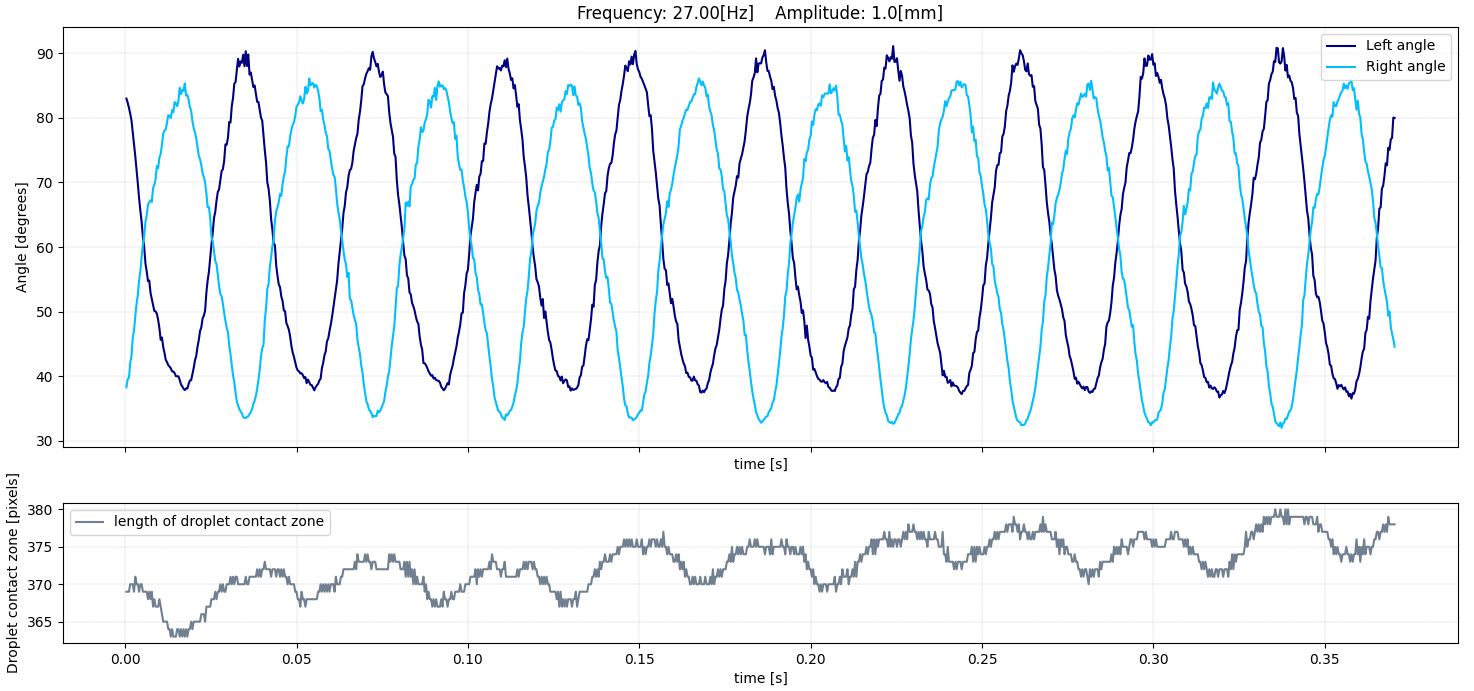
\includegraphics[width=1\textwidth]{../workspace/a10_f135z.png} 
\end{center}
\caption{Charakterystyka kątów zwilżania dla sinusoidalnego wymuszenia ruchu.  \\Amplituda drgań: 1.0 mm,  częstotliwość: 27 Hz.}
\label{fig:theta(t)_5}
\end{figure} 
\newpage

\captionsetup{skip=0pt}
\begin{figure}[!h]
\captionsetup{justification=centering}
\begin{center}
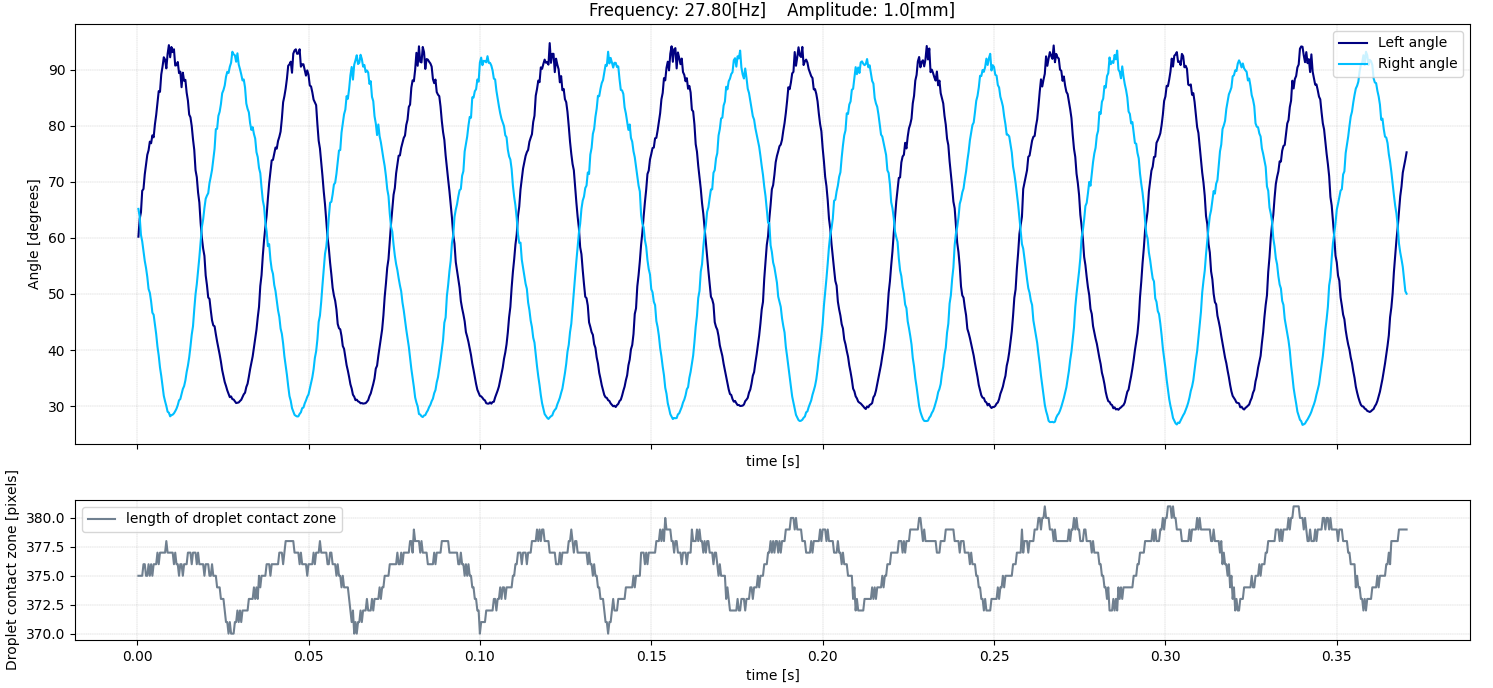
\includegraphics[width=1\textwidth]{../workspace/a10_f139z.png} 
\end{center}
\caption{Charakterystyka kątów zwilżania dla sinusoidalnego wymuszenia ruchu.  \\Amplituda drgań: 1.0 mm,  częstotliwość: 27.8 Hz.}
\label{fig:theta(t)_6}
\end{figure} 

\captionsetup{skip=0pt}
\begin{figure}[!h]
\captionsetup{justification=centering}
\begin{center}
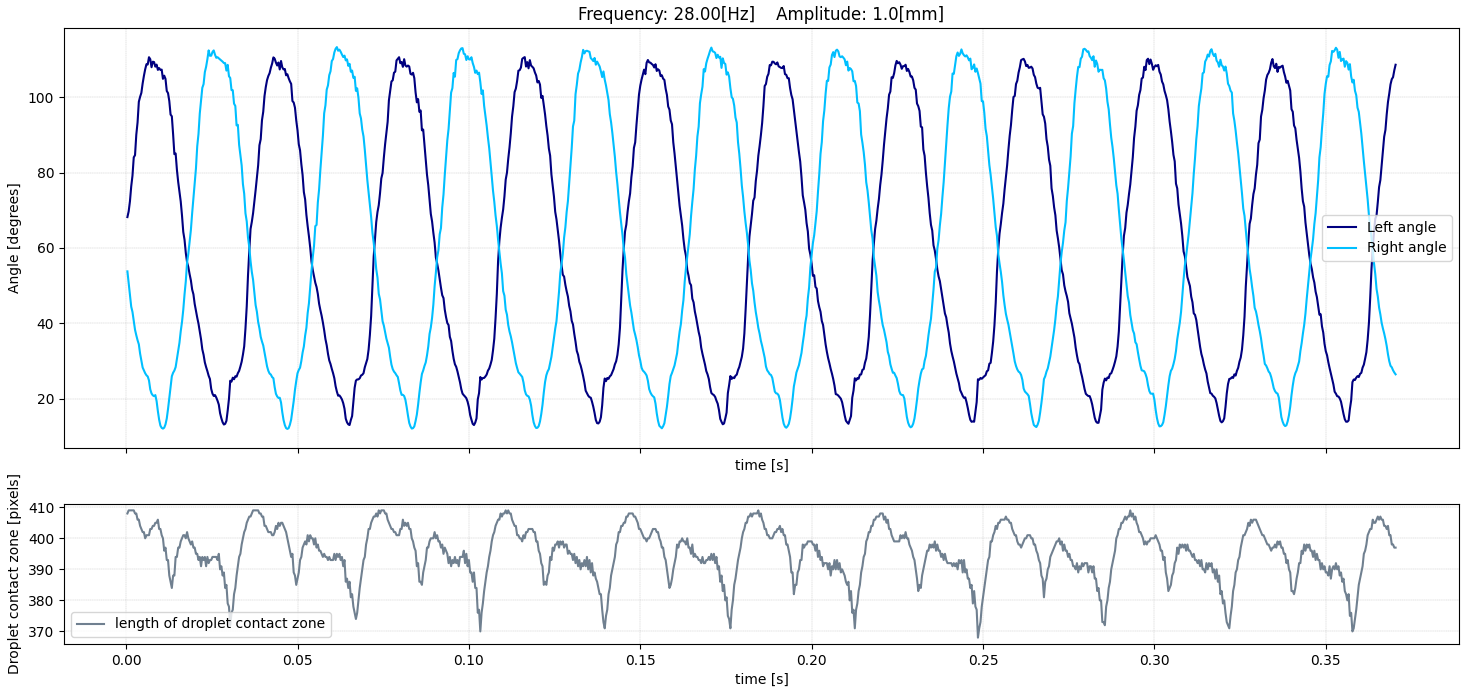
\includegraphics[width=1\textwidth]{../workspace/a10_f140z.png} 
\end{center}
\caption{Charakterystyka kątów zwilżania dla sinusoidalnego wymuszenia ruchu.  \\Amplituda drgań: 1.0 mm,  częstotliwość: 28 Hz.}
\label{fig:theta(t)_7}
\end{figure} 

\vspace{5mm}
\noindent W przypadku większych częstotliwości drgań (rys. \ref{fig:theta(t)_7}) przebiegi są zdecydowanie bardziej wygładzone. Obserwacja długości strefy kontaktu pozwala na identyfikację tego, czy w danym pomiarze występuje poślizg. Dalszy rozwój algorytmu przewiduje uwzględnienie tej własności poprzez wykluczenie pomiarów, w których dochodzi do poślizgu. 
\newpage

\subsection{Wartości maksymalne, minimalne i średnie na podstawie charakterystyk kątów zwilżania}
\noindent Dane przedstawione na wykresach (\ref{fig:theta(t)_1} - \ref{fig:theta(t)_7}) można zbiorczo podsumować na wykresach przedstawiających wartość średnią kąta i odpowiadającą jej wartość maksymalną oraz minimalną w funkcji częstotliwości wymuszenia. Wykresy te sporządzono dla wszystkich danych pomiarowych. Wartość średnią kątów zwilżenia obliczono ze wzoru:
\begin{equation}
\theta_{\text{AVG}} = \cfrac{1}{T} \int_0^T \theta(t) dt
\end{equation}
\noindent gdzie T oznacza przedział czasowy, w którym liczona jest wartość średnia. Częstotliwość, dla której doszło do wyraźnego uślizgu kropli uznano jako częstotliwość graniczną, powyżej której kropla zawsze ulegnie poślizgowi. Obszar ten wyszczególniono poprzez jego zakreślenie. 

\captionsetup{skip=0pt}
\begin{figure}[!h]
\captionsetup{justification=centering}
\begin{center}
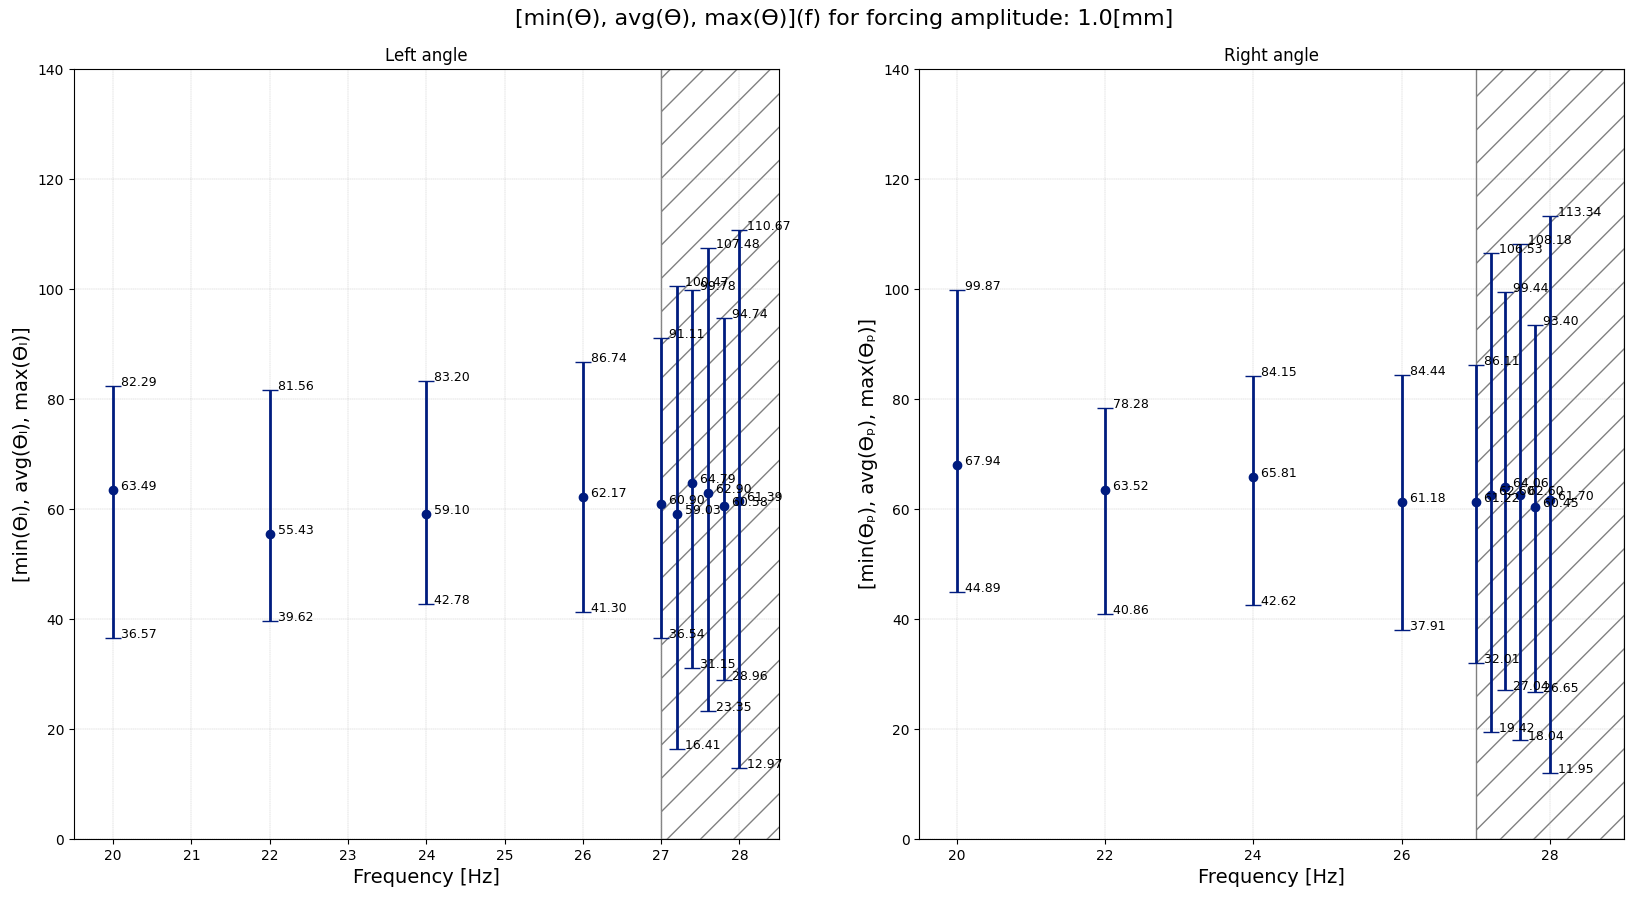
\includegraphics[width=1\textwidth]{../workspace/MinMaxAvg1.0.png} 
\end{center}
\caption{Dyskretny rozkład $\theta_{min}, \theta_{avg}, \theta_{max}$ dla określonych częstotliwości wymuszenia. \\Lewy wykres odpowiada wielkościom charakteryzującym lewy kąt, natomiast\\ na prawym wykresie zestawiono odpowiadające wielkości dla kąta prawego.}
\label{fig:MinMaxAvg1}
\end{figure} 

\vspace{4mm}
\noindent Przedstawiony wykres wskazuje na to, że w momencie uślizgu wzrastają skrajne wartości kąta ($\theta_{min}$, $\theta_{max}$). Nie zmienia się natomiast zauważalnie wartość średnia kąta ($\theta_{\text{AVG}}$). Zależność tę zaobserwowano także dla pozostałych danych pomiarowych (rys. \ref{fig:MinMaxAvg2} - rys. \ref{fig:MinMaxAvg3})

\newpage
\noindent Analogiczne wykresy sporządzono dla amplitud wymuszenia wynoszących odpowiednio 2.0 oraz 3.0 mm (rys. \ref{fig:MinMaxAvg2} - rys. \ref{fig:MinMaxAvg3})
\captionsetup{skip=0pt}
\begin{figure}[!h]
\captionsetup{justification=centering}
\begin{center}
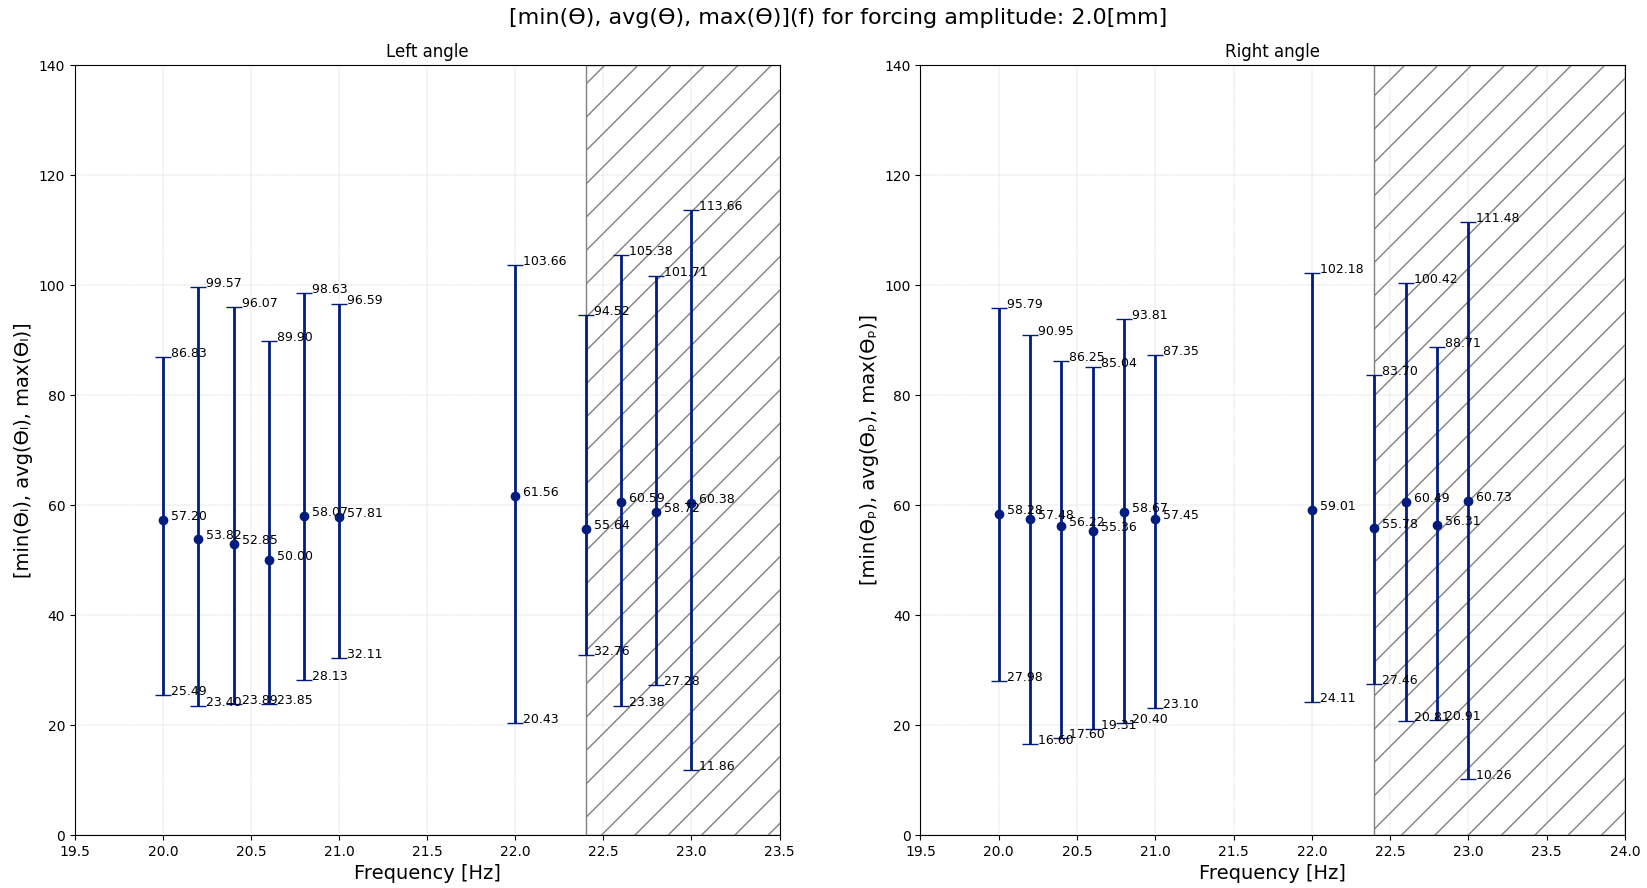
\includegraphics[width=1\textwidth]{../workspace/MinMaxAvg2.0.png} 
\end{center}
\caption{Dyskretny rozkład $\theta_{min}, \theta_{avg}, \theta_{max}$ dla określonych częstotliwości wymuszenia.\\Amplituda wymuszenia: 2.0 mm.}
\label{fig:MinMaxAvg2}
\end{figure} 


\captionsetup{skip=0pt}
\begin{figure}[!h]
\captionsetup{justification=centering}
\begin{center}
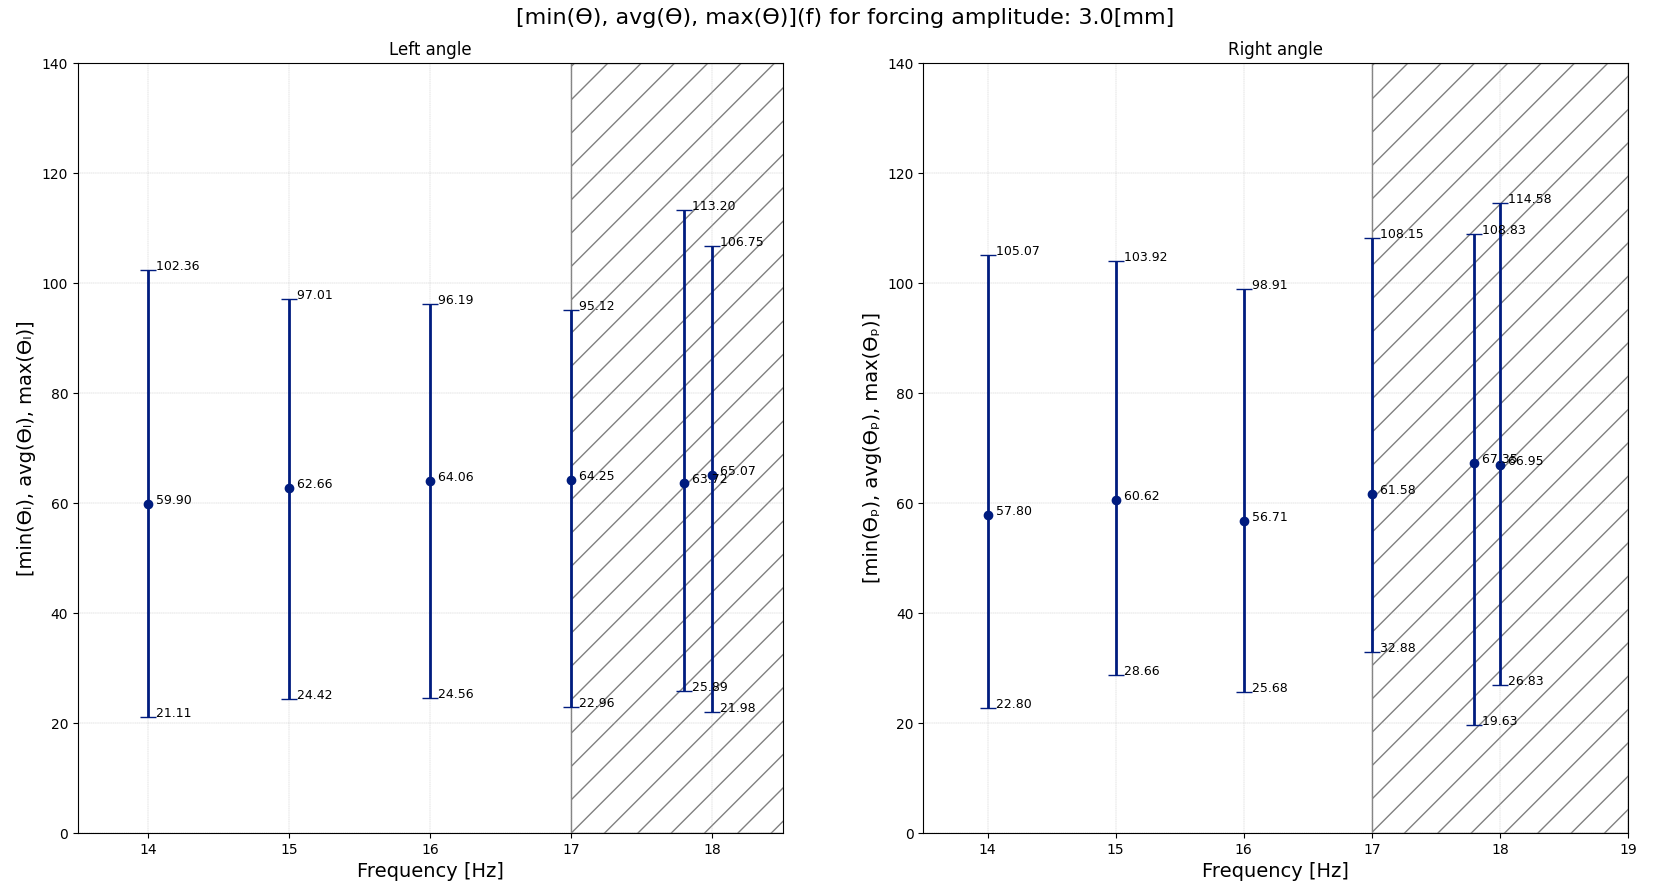
\includegraphics[width=1\textwidth]{../workspace/MinMaxAvg3.0.png} 
\end{center}
\caption{Dyskretny rozkład $\theta_{min}, \theta_{avg}, \theta_{max}$ dla określonych częstotliwości wymuszenia. \\Amplituda wymuszenia: 3.0 mm.}
\label{fig:MinMaxAvg3}
\end{figure} 

\newpage
\section{Transformacja Fouriera} \label{chapter:fourier}
\noindent Analiza Fouriera to metoda wyrażania funkcji jako sumy składowych okresowych oraz odzyskiwania sygnału z tych składowych. Kiedy zarówno funkcja, jak i jej transformata Fouriera są zastępowane dyskretnymi odpowiednikami, nazywa się to dyskretną transformatą Fouriera (DFT). Dyskretna transformata Fouriera jest odpowiednikiem ciągłej transformaty Fouriera dla sygnałów znanych tylko w chwilach oddzielonych od siebie czasami próbkowania (tj.
skończonego ciągu danych). Niech f(t) będzie sygnałem ciągłym, który jest źródłem danych. Oznaczmy także N próbek jako  f[0], f[1], f[2], ..., f[k], ..., f[N-1]. Transformację Fouriera sygnały wyjściowego można wtedy zapisać jako \cite{HJNus}:
\begin{equation}
F(j \omega) = \int_{-\infty}^{\infty} f(t) e^{-j \omega t }dt
\end{equation}
\noindent Każdą próbkę możemy traktować jako impuls mający powierzchnię f[k] \cite{HJNus}. W takim razie, biorąc pod uwagę, że całka istnieje tylko w punkcie próbkowania możemy zapisać, że:
\begin{equation}
F(j \omega) = \int_{0}^{(N-1)T} f(t) e^{-j \omega t }dt = f[0]e^{-j 0} + f[1]e^{-j \omega T} + ... + f[k]e^{-j \omega t} + ... +  f(N-1) e^{-j \omega (N-1) T }
\end{equation}
\noindent Co możemy przekształcić do postaci \cite{Rao}:
\begin{equation}
F(j\omega) = \sum_{k=0}^{N-1} f[k] e^{-j \omega k T}
\end{equation}

\noindent Ponieważ istnieje tylko skończona liczba punktów danych wejściowych, DFT traktuje dane tak, jakby były okresowe (tj. f[N] do f[2N-1] jest takie samo jak f[0] do f[N-1]). Ze względu na to, że operacja traktuje dane tak, jakby były okresowe, rozwija się równanie DFT dla częstotliwości podstawowej (jeden cykl na sekwencję $\frac{1}{NT}$ Hz, $\frac{2 \pi}{NT}$ rad/sec) i jego harmoniczne do postaci \cite{Rao}:
\begin{equation} \label{eq:DFT}
F[n] = \sum^{N-1}_{k=0}f[k]e^{-j \frac{2 \pi}{N}nk}   \quad (n=0 : N-1)
\end{equation}

\noindent  Algorytmem do wyznaczania dyskretnej transformaty Fouriera oraz transformaty do niej odwrotnej jest FFT (\textit{ang. Fast Fourier Transform}). Obliczanie sum za pomocą wzoru (\ref{eq:DFT}) wymaga wykonania O($N^2$) operacji. FFT można zdefiniować jako DFT ze zmniejszoną liczbą niezbędnych operacji arytmetycznych. Celem FFT jest zmniejszenie długiego algorytmu obliczeniowego przez jego podział na krótsze i prostsze obliczenia DFT. Istnieją różne algorytmy FFT. Złożoność obliczeniowa szybkiej transformacji Fouriera wynosi O($N\log_2 N$). Realizację FFT zapewniono poprzez implementację dostępnej w bibliotece \textbf{SciPy} jednowymiarowej, dyskretnej transformacji opracowanej przez Cooley'a i Tokey'a \cite{FFT_cooley}.

\newpage




\newpage
\begin{thebibliography}{99}
\bibitem{ALGEBRA}
\text{Roger A. Horn, Charles R. Johnson, ''Topics in Matrix Analysis'' }\\
\text{Cambridge University Press, March 2011}


\bibitem{FFT_cooley}
\text{Cooley, James W., and John W. Tukey, 1965,}\\
\text{ “An algorithm for the machine calculation of complex Fourier series,”}\\
\text{ Math. Comput. 19: 297-301.}

\bibitem{HJNus}
\text{H. J. Nussbaumer, ''Fast Fourier Transform and Convolution  Algorithms''.}\\
\text{Springer Series in Information Sciences, 1982}

\bibitem{Rao}
\text{K. R. Rao, D. N. Kim, J.J. Hwang}\\
\text{ ''Fast Fourier Transform: Algorithms and Applications''}\\
\text{Springer Dordrecht Heidelberg London New York, 2010}



\end{thebibliography}




\end{document}
